% --------------------------------------------------------------------------- %
% --------------------------------------------------------------------------- %
\chapter{The LHC Accelerator and CMS Experiment}
\label {ch:cms}

The Compact Muon Solenoid (CMS) experiment is a collaboration of scientists
working together to investigate the data streaming from the Large Hadron
Collider (LHC). This chapter will give an overview of the experimental setup
used by the nearly 3,000 CMS collaborators to analyze this data. First 
we give a short discussion of the Large Hadron Collider followed by
the Compact Muon Solenoid detector itself. Finally, we will give a brief
description of the algorithms used to measure the particles traversing the CMS
detector used by the various analyses.

% --------------------------------------------------------------------------- %
% --------------------------------------------------------------------------- %
\section{The Large Hadron Collider}
\label {sec:cms_lhc}
% --------------------------------------------------------------------------- %
% --------------------------------------------------------------------------- %

As previously discussed in Chapter~\ref{ch:intro}, the Standard Model of
particle physics (SM) is the de facto theory that currently describes all
known particle interactions save gravity. The aim of the Large Hadron Collider
(LHC) is to invesitage the possibility of physics beyond the Standard Model.
Completed in 2008, it is approximately 27 km in circumference, sits 170
meters underground and was designed to accelerate protons to 7 \TeV~each and
collide them at four interaction points. Each interaction point has a detector
positioned there to record the outcome of these proton-proton collisions: the
two general purpose detectors CMS and ATLAS, and the other two specialized
detectors ALICE and LHC-b. Figure \ref{fig:cms_underground}~shows a cartoon of
the LHC and the four particle detectors which is located on the outskirts of
Geneva, Switzerland.

% --------------------------------------------------------------------------- %
\begin{figure}[tbhp]
\centering
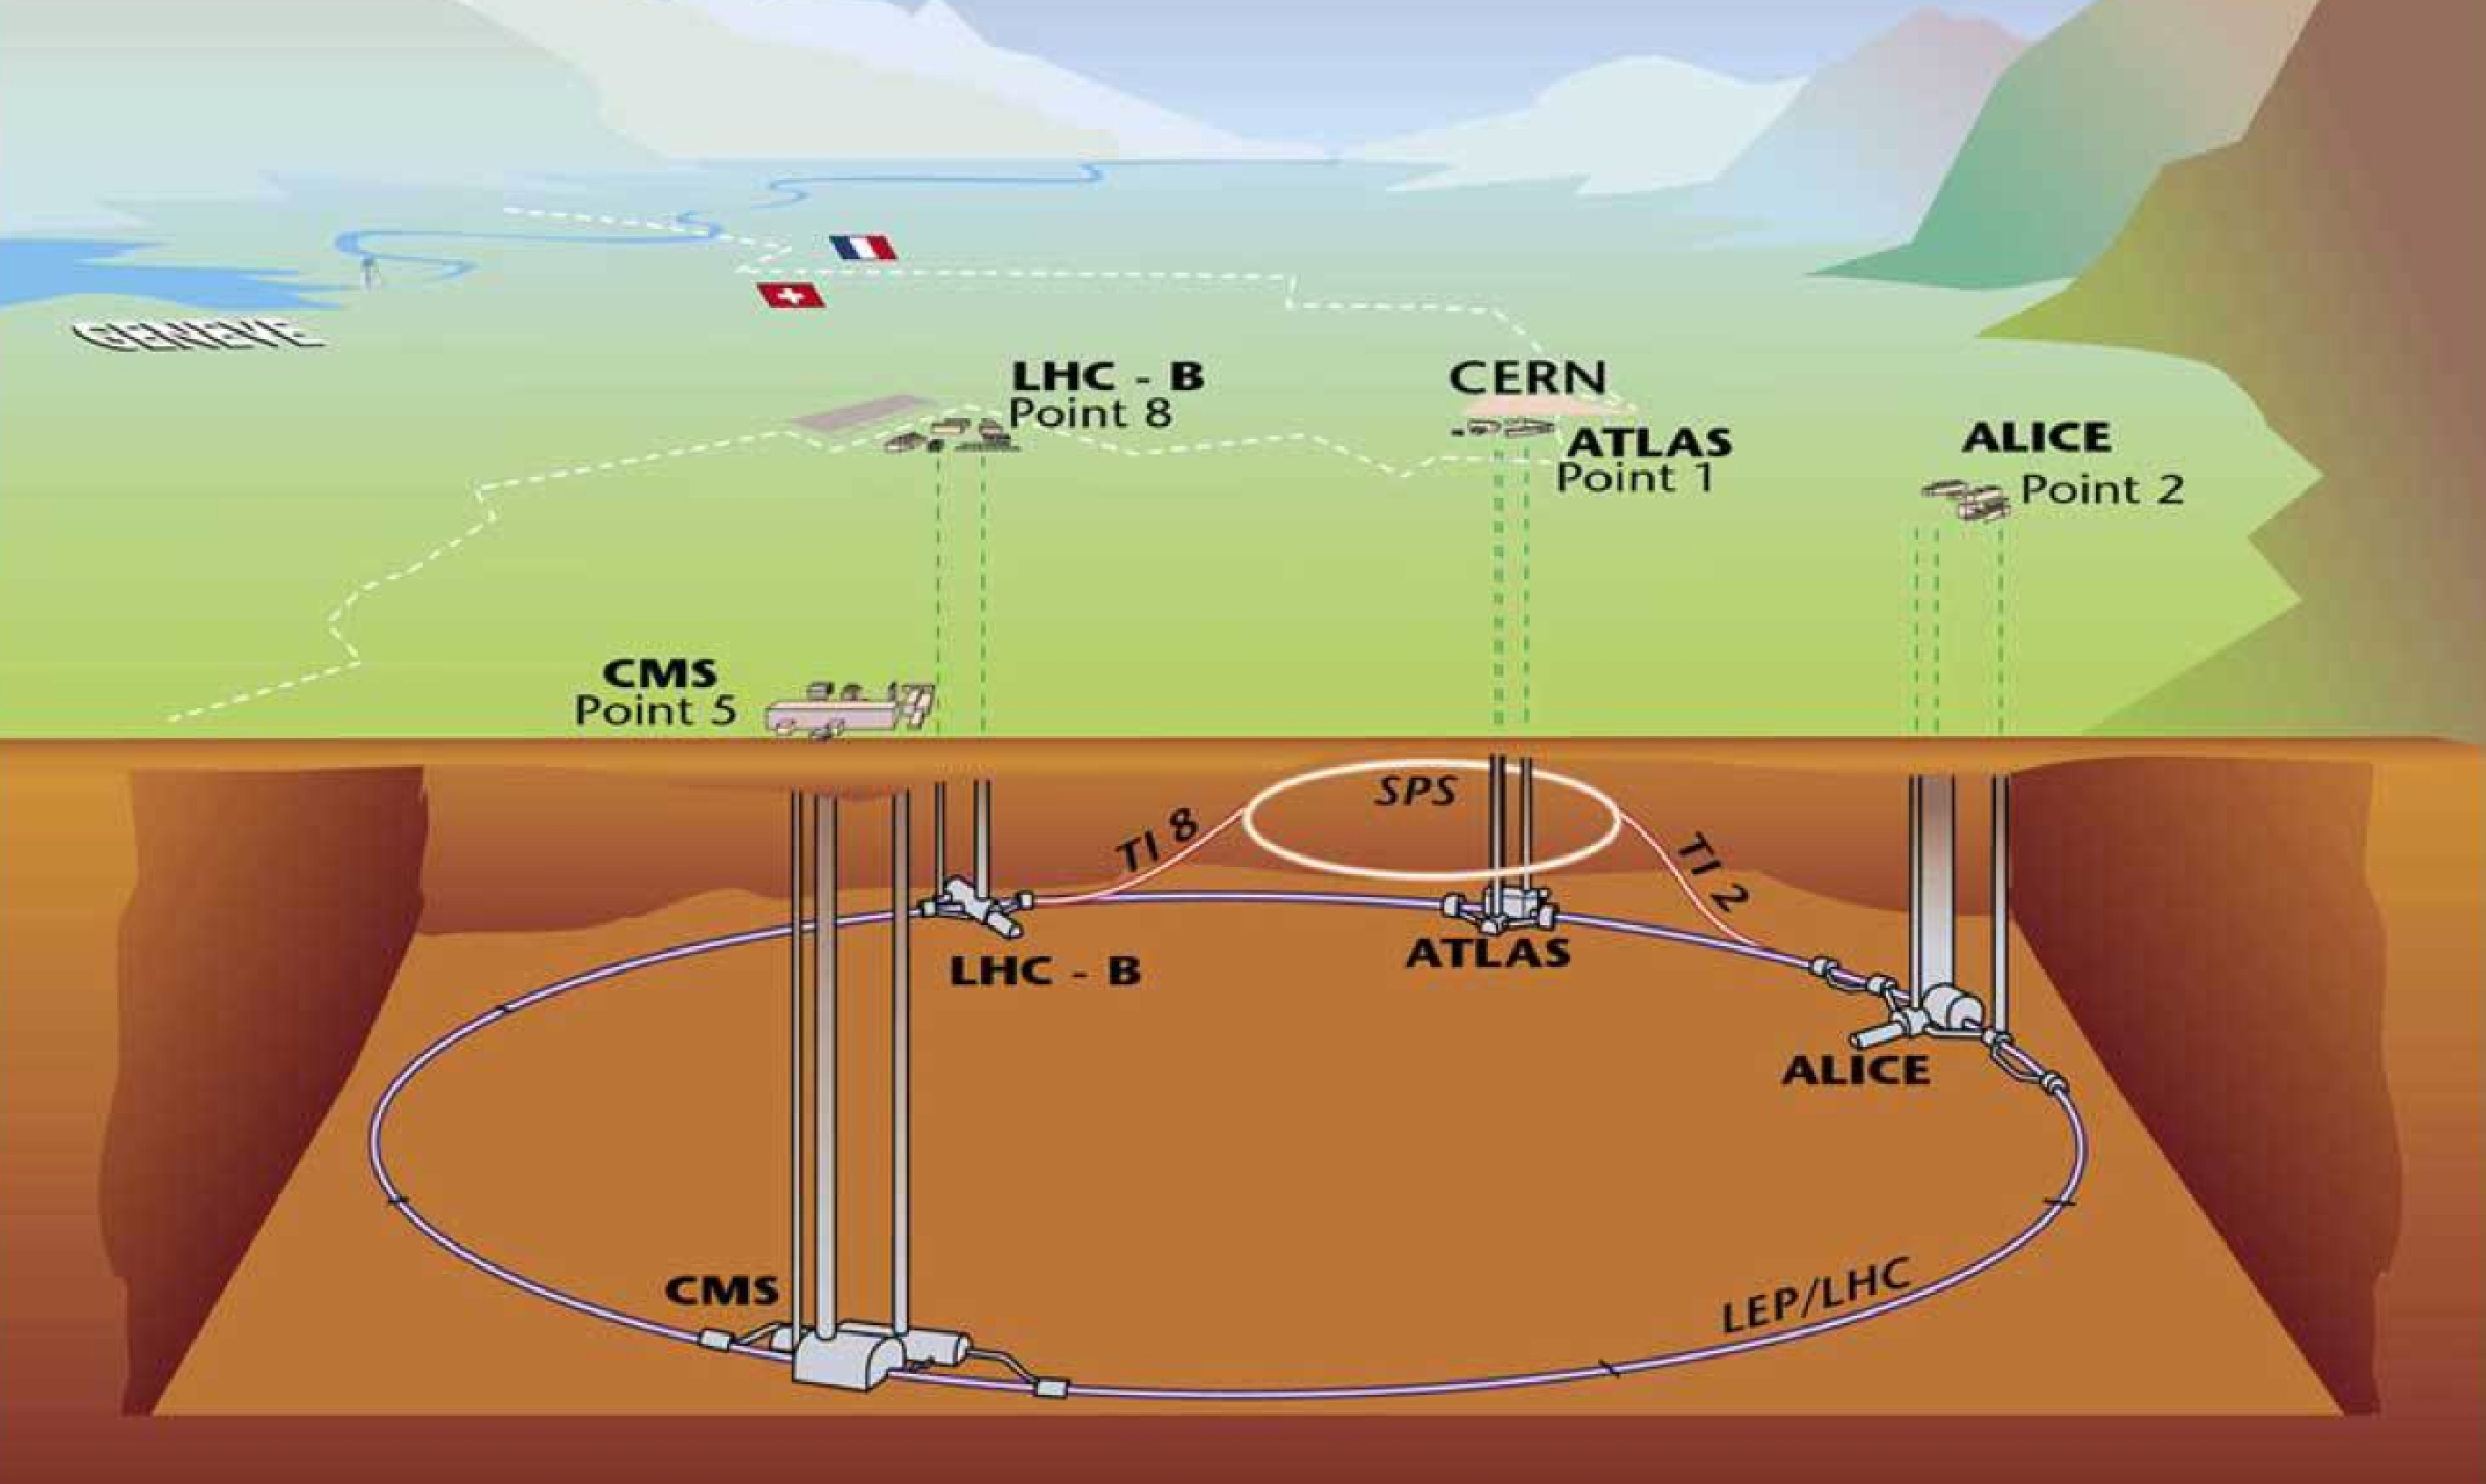
\includegraphics[width=0.9\textwidth]{underground.pdf}
\caption[The Large Hadron complex seen underground on the outskirts of  Geneva, Switzerland]
{\label{fig:cms_underground}
The Large Hadron complex seen underground on the
outskirts of Geneva, Switzerland. The four detectors main detectors are also shown -- LHC-B, ATLAS, ALICE, and, most
relevant to this analysis, CMS at Point 5~\cite{lhcmachine}.
}
\end{figure}
% --------------------------------------------------------------------------- %

The search for the Higgs boson carried a large influence on the design of
the Large Hadron Collider (LHC) and the CMS detector. The previously unknown
mass of the Higgs boson combined with its small production cross section
required building a machine capable of high energy collisions at a high rate.
This design leads to approximately 1 billion proton-proton collisions per
second~\cite{lhcmachine}. Rather than continuous beams, the protons will be
``bunched'' together, into 2,808 bunches, 115 billion protons in each bunch so
that interactions between the two beams will take place at discrete intervals
never shorter than 25 nanoseconds (ns) apart. The design luminosity of the LHC
is $10^{34} \rm{cm^{−2}s^{−1}}$, providing a bunch collision rate of 40 MHz.

Although the design center-of-mass energy ($\sqrt{s}$) is 14 TeV, the data 
collected from 2011 and 2012 was at $\sqrt{s} = 7\ \TeV$ and $8\ \TeV$, respectively.
The data used for this thesis is the full dataset recorded from 2012 at 
$\sqrt{s} = 8\ \TeV$. The LHC plans to continue collisions in 2015 at $\sqrt{s}
= 13\ \TeV$.

% --------------------------------------------------------------------------- %
% --------------------------------------------------------------------------- %
\section{The Compact Muon Solenoid Detector}
\label {sec:cms_cms}
% --------------------------------------------------------------------------- %
% --------------------------------------------------------------------------- %
The Compact Muon Solenoid (CMS) is one of the two general purpose detectors
situated along the beam line of the LHC. The name ``compact'' comes from
the fact that the detector is relatively small when compared to it's
sister experiment known as A Toroidal LHC Apparatus (ATLAS); however, CMS
is by no means small. Weighing in at over 12,000 tons, cylindrical in
shape, it is over 21 meters in length and 14 meters in diameter. It sits
$\sim$100 meters underground at LHC Point 5 near Cessy, France (see Figure
\ref{fig:cms_underground}). An overview of the CMS detector can be seen in
Figure \ref{fig:cms_diag}.
% --------------------------------------------------------------------------- %
\begin{figure}[tbhp]
\centering
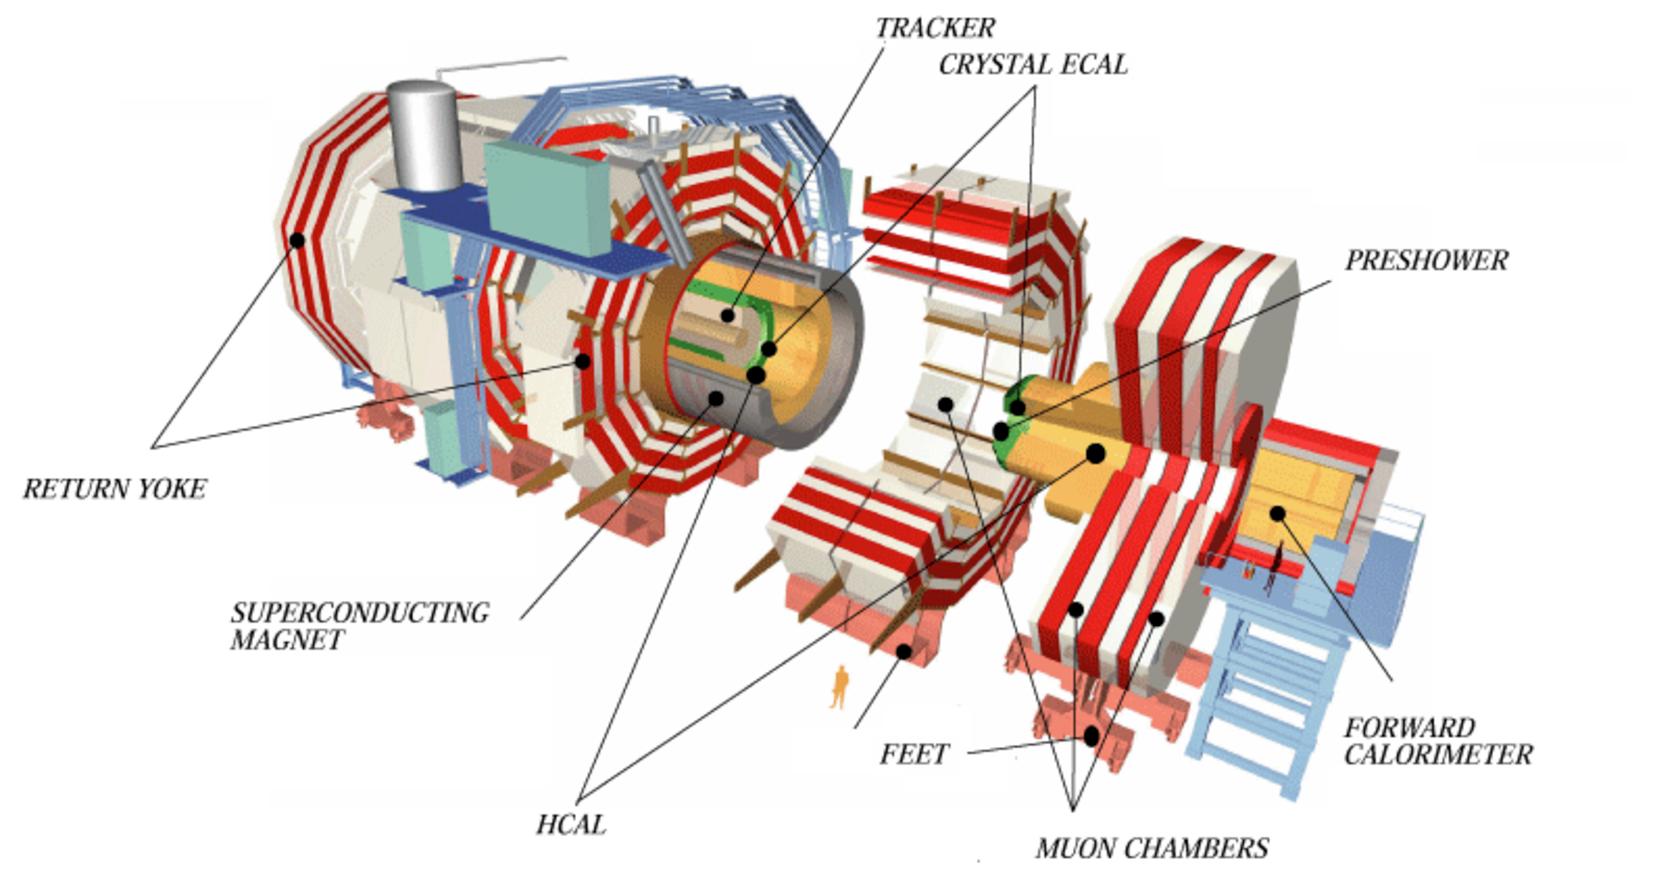
\includegraphics[width=0.9\textwidth]{cms_diag.pdf}
\caption[Overview of the Compact Muon Solenoid detector]
{\label{fig:cms_diag}
Overview of the Compact Muon Solenoid detector~\cite{cmspic}.
}
\end{figure}
% --------------------------------------------------------------------------- %
CMS was designed to allow for the study of many different unanswered questions
in particle physics. To achieve this broad objective, CMS is capable of
measuring with high precision, the trajectory, momentum and energy of many
different types of particles. In addition, it is able to handle the challenging
conditions presented by the high luminosity and high energy collisions from
the LHC. To deal with the approximately one billion interactions per second
expected from the LHC at its design luminosity, CMS is a very high granular
detector, and hence has many electronic channels, each with excellent time
resolution and is designed to be radiation hard to deal with the multitude of
particles produced during each bunch crossing.

CMS contains a strong magnetic field produced by a superconducting solenoid.
An inner field strength of 3.8 Tesla ensures that even the highest momentum
particles propagating through the detector have enough curvature to ensure a
precise momentum measurement. Inside the solenoid sit both the silicon and
pixel tracker systems and both the electromagnetic (ECAL) and hadronic
calorimeters (HCAL). The larger number of channels in the pixel tracker
ensure a precise measurement of the origin of particles both produced near
the beamline and those with longer lifetimes decaying at larger diameters.
The silicon strip detector has at least 10 layers along any particles' path
allowing precise particle ``tracking'' and momentum measurements. The ECAL,
with over 75,000 lead-tungstate (\pbw) scintillating crystals, gives
excellent energy measurements of the particles which interact primarily
electromagnetically, namely electrons and photons. The HCAL, a sampling
calorimeter made of brass, completes the sub-detectors existing inside of the
solenoid and gives respectable energy resolution for particles that interact
primarily hadronically (e.g. pions and kaons).

Outside of the solenoid rests the final major sub-detector, the muon detector.
Made up of three separate components, the muon chambers are placed between the large
iron frame (yoke) that serves two purposes. First, they prevent particles
other than muons from reaching the outermost muon chambers and hence allow for
excellent muon identification. Secondly, the yoke allows for a strong return
magnetic field to fill the entirety of the muon detector system which allows
for better momentum resolution.

The coordinate system of CMS is centered at the nominal interaction point at
the center of CMS's cylindrical shape. We define the y-axis to point upwards
(away from the center of the earth), the x-axis the points towards the center
of the LHC ring and hence, the z-axis points along the beamline, counter
clockwise around the LHC. The azimuthal angle, $\phi$, is measured from the
zero position of the x-axis in the x-y plane while the polar angle, $\theta$, is
measured from the positive z-axis.

Finally, we should introduce now two important quantities used in hadronic
collider physics. While we know precisely the center-of-momentum frame
and individual momenta of the two colliding protons, we do not know the
center-of-momentum frame for the two colliding partons. For this reason, we
define two quantities that are invariant under a boost in the direction of the
proton's momentum. The first quantity is the partons' momentum in the plane
normal to the collision -- i.e. the transverse plane, the transverse momentum
(\pt) can be defined and is, to first order, conserved. The second quantity,
pseudorapidity ($\eta$) is a transformation from the polar angle into an
invariant quantity with respect to the frame of the collision:

% ---------------------------------------------------------------------------
\begin{equation}
    \eta = - \rm{ln} \left[\rm{tan}\left(\frac{\theta}{2}\right)\right],
\end{equation}
% ---------------------------------------------------------------------------
where $\theta$ is the angle between the incoming proton and the outgoing
particle. These two quantities, \pt and $\eta$, are used extensively at the
LHC to describe the kinematics of the out going particles from a proton-proton
collision and will be used throughout this analysis as well.

A complete description of the CMS detector can be found in Reference~\cite{jinst},
from which all information in this section is derived, unless explicitly
stated. The following subsections give a more detailed description of the various
pieces that make up the CMS detector. This is not meant to be a full detector
description; however, we do highlight details that are important to the
analysis in this thesis.

% --------------------------------------------------------------------------- %
% --------------------------------------------------------------------------- %
\subsection{The Superconducting Solenoid}
\label {sec:cms_solenoid}
% --------------------------------------------------------------------------- %
% --------------------------------------------------------------------------- %
Charged particles in an electromagnetic field experience a force given by
\[
\mathbf{F} = q\left(\mathbf{E} + \mathbf{v}\times\mathbf{B}\right),
\]
where q is the charge of the paricle, $\mathbf{E}$ is the electric field,
$\mathbf{v}$ is the velocity of the charged particle and $\mathbf{B}$ is
the magnetic field. Therefore, for a uniform magnetic field, the radius of
curvature, r, of a charge particles is directly proportional to the particle's
momentum and inversely proportional to the magnetic field strength,
\[
r = \frac{\pt}{q |\mathbf{B}|},
\]
where \pt is the particles transverse momentum with respect to the direction
of the magnetic field. With $\sim$3 meters from the nominal interaction point
to the inside edge of the solenoid, CMS must have a strong magnetic field to
achieve the maximum possible curvature for the charged particles. This ensures
the most precise measurement of the momentum and this is achieved with CMS's
superconducting solenoid.

Made up of Niobium-Titanium ($\rm NbTi$), the solenoid was designed to operate
with a magnetic field strength of 4 Tesla, yet due to safety considerations,
is operated at 3.8 Tesla. At maximum strength, the solenoid stores over 2
Gigajoules of energy and far exceeds the design strength of all other particle
detectors.

To allow for this stronger magnetic field, and hence better momentum
measurement, for the muon chambers, the outside of the solenoid has been
designed with iron yokes which offer integral support, provide additional
stopping power for non-muons and propagates the magnetic field. The yokes can
be seen in red in Figure~\ref{fig:cms_diag}.

% --------------------------------------------------------------------------- %
% --------------------------------------------------------------------------- %
\subsection{The Silicon Detector}
\label {sec:cms_silicon}
% --------------------------------------------------------------------------- %
% --------------------------------------------------------------------------- %
The innermost portion of the CMS detector is comprised of a silicon based
particle tracking system (tracker). Doped and negatively biased, when charged
particles traverse the active region of the silicon, electric current is
induced and measured. This gives a positional measurement of the charged
particles and is recorded for later reconstruction (hits). Combining the
multiple positional measurements, the curvature of a charged particle is
measured, and thus, using the known magnetic field strength, the particle's
momentum. The tracker was designed to have a high efficiency to properly
reconstruct the trajectory, good momentum resolution and be able to identify
secondary vertices from longer lived particles such as b-flavored hadrons.

Many aspects of the tracker were specifically tailored to achieve the design
considerations discussed above and to physically fit within the CMS solenoid.
First, in order to deal with large particle multiplicities, the detector needed
to be radiation hard, have a high granularity and a fast electronic response
time. The high granularity was achieved by using a pixel silicon detector in the
inner most region. Outside of the pixel detector, silicon strips are used as
the particle multiplicity density decreases as the square of the radius from
the interaction point. This design achieves the desired position, momentum
and vertex resolution while keeping the occupancy down to a manageable 1\%
throughout. An overview of the layout of the silicon tracker can be see in
Figure~\ref{fig:cms_tracker} with the following subsections discussing the
pixel and strip detectors, respectively.
% --------------------------------------------------------------------------- %
\begin{figure}[tbhp]
\begin{center}
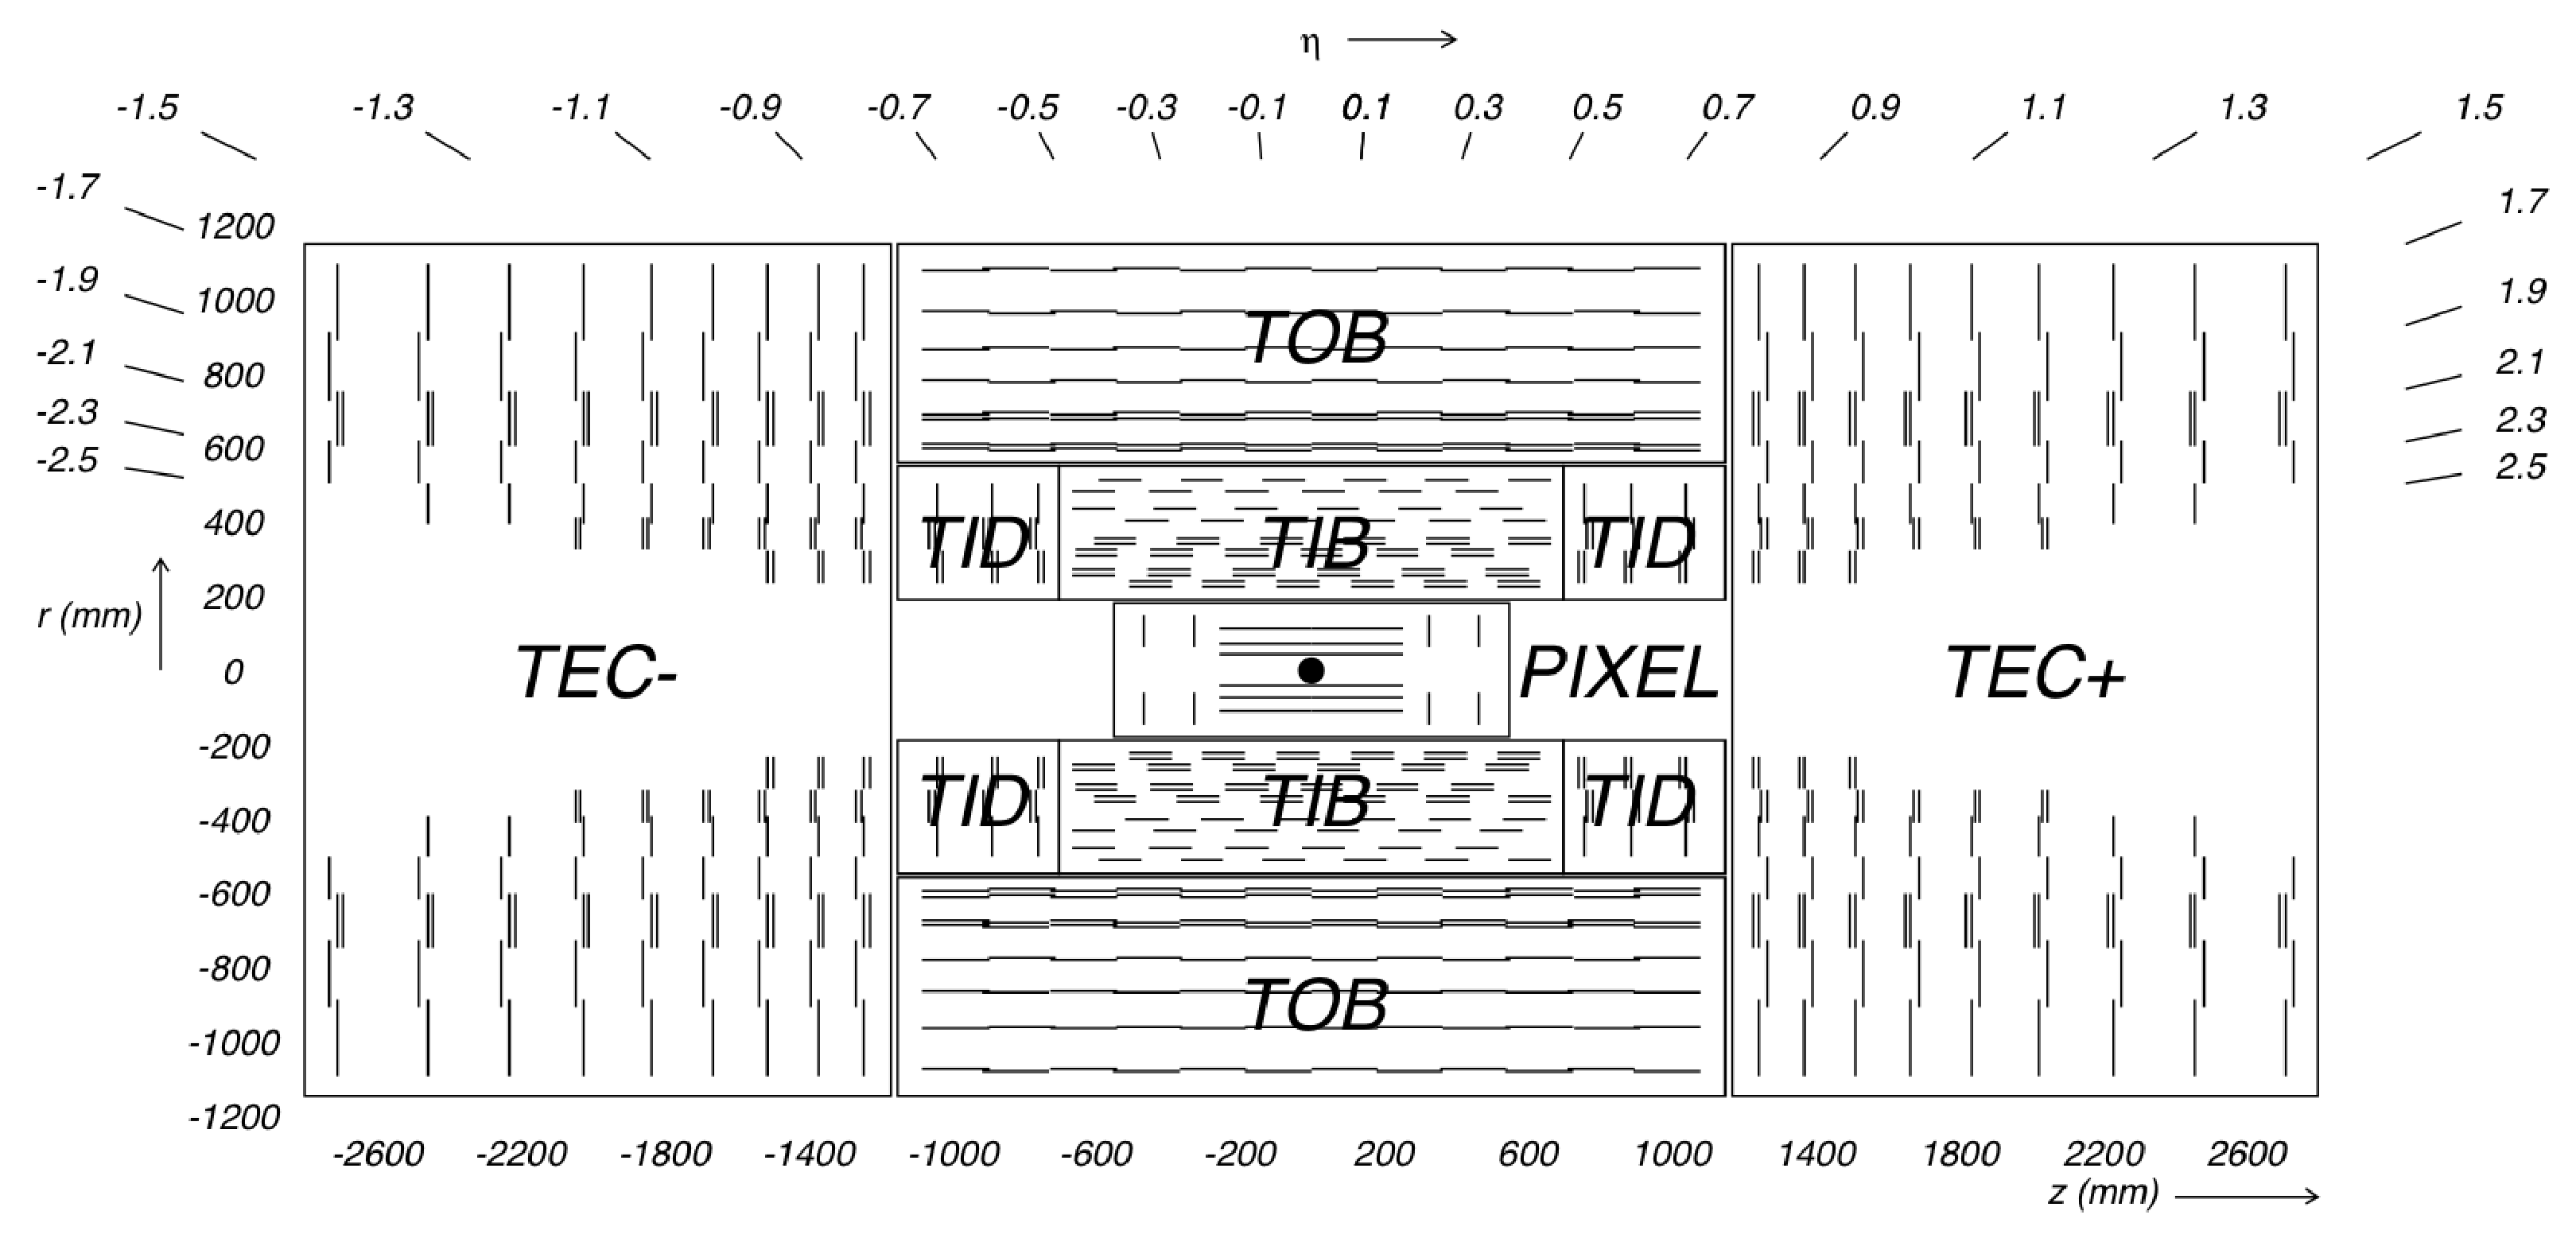
\includegraphics[width=0.95\textwidth]{tklayout.pdf}
\caption[Layout of the tracking system projected into the $rz$ plane]
{\label{fig:cms_tracker}
Layout of the tracking system projected into the $rz$ plane. Modules are
shown as lines and modules with back-to-back labels appear as double parallel
lines~\cite{trackingperformance}.
}
\end{center}
\end{figure}
% --------------------------------------------------------------------------- %

\subsubsection{The Pixel Detector}
\label {sec:cms_silicon_pixel}

In order to achieve the 1\% occupancy nearest the beam line, pixel silicon
detectors are used within a radius of $\sim$10 \cm. The CMS pixel detector
consists of three concentric cylindrical layers at 4.4, 7.4 and 10.2 \cm in
the radial direction with two disks at 34.5 and 45.6 \cm on each side along
the z-coordinate. Together, the ``barrel'' and ``endcap'' pixel detectors
cover a pseudorapidity range up to $\aeta < 2.5$. The pixels themselves
are approximately square with a size of 100 to 150 \um per side and have a
spatial resolution of 10 \um in the $r - \phi$ direction and 200 \um in the
z direction. Besides allowing for low occupancy, the pixel detectors are
also be made radiation hard and are designed to give precise vertex position
measurements.

\subsubsection{The Strip Detector}
\label {sec:cms_silicon_strip}

Outside of the pixel detector sits the silicon strip detector. At these
distances from the interaction point, a lower density of sensors can be
used to obtain the same occupancy. Strip detectors (long rectangular
active regions) are significantly cheaper to manufacture than pixel detectors
while still providing the desired momentum resolution and channel occupancy.
The strip detector can be divided into four different regions: the tracker
inner barrel (TIB), the tracker inner disks (TID), the tracker outer
barrel (TOB) and the tracker endcaps (TEC). Each region can be seen in
Figure~\ref{fig:cms_tracker}. The TIB consists of four cylindrical layers
in the barrel and is surrounded on each side by three disks from the TID. The
TIB and TID extend out to a radius of approximately 55 \cm and provide
position measurement resolution of between 23 and 35 \um. The TOB surrounds the
TIB and TID and provides another 6 cylindrical layers and provides slightly
less resolution of around 35 to 53 \um. Finally, the TEC extends out into the
z-direction by providing an additional 9 disk layers with resolution between 97
and 184 \um. The silicon strip detector also provides a pseudorapidity coverage
inside $\aeta < 2.5$. Some of the layers in the strip detector, namely the first
two layers in each TIB, TID, TOB and TEC as well as layer five in the TEC,
carry an additional offset detector mounted at a slight angle. This allows not
just for additional positional measurement but an additional measurement in the
``non-strip'' direction (z in the barrel and r in the endcaps).

\subsubsection{The Tracker}
\label {sec:cms_silicon_tracker}

With over 200 square meters of silicon, the CMS Tracker is the largest silicon
detector in the world. Unfortunately, material comes at a performance cost.
The silicon must all the powered, and in turn, the powered units must all
be cooled (operating temperate is $-10\ ^{\circ}\mathrm{C}$). The amount
of material in the CMS tracker is shown in units of radiation length in
Figure~\ref{fig:cms_material}. A radiation length is a characteristic of a
material and describes the distance over which electrons and photons lose
energy and is the length at which an electron, on average, will lose all but
$1/e$ of its initial energy via bremsstrahlung. All of this material inside CMS
causes a few complications. First, particle momentum resolution is degraded as
each particle has a higher probability for nuclear interaction and multiple
scattering as it traverses the detector. Second, electrons and photons have higher
probabilities to bremsstrahlung and pair create, respectively, causing issues
measuring their energy in the electromagnetic calorimeter (see next section).
% --------------------------------------------------------------------------- %
\begin{figure}[!htb]
\begin{center}
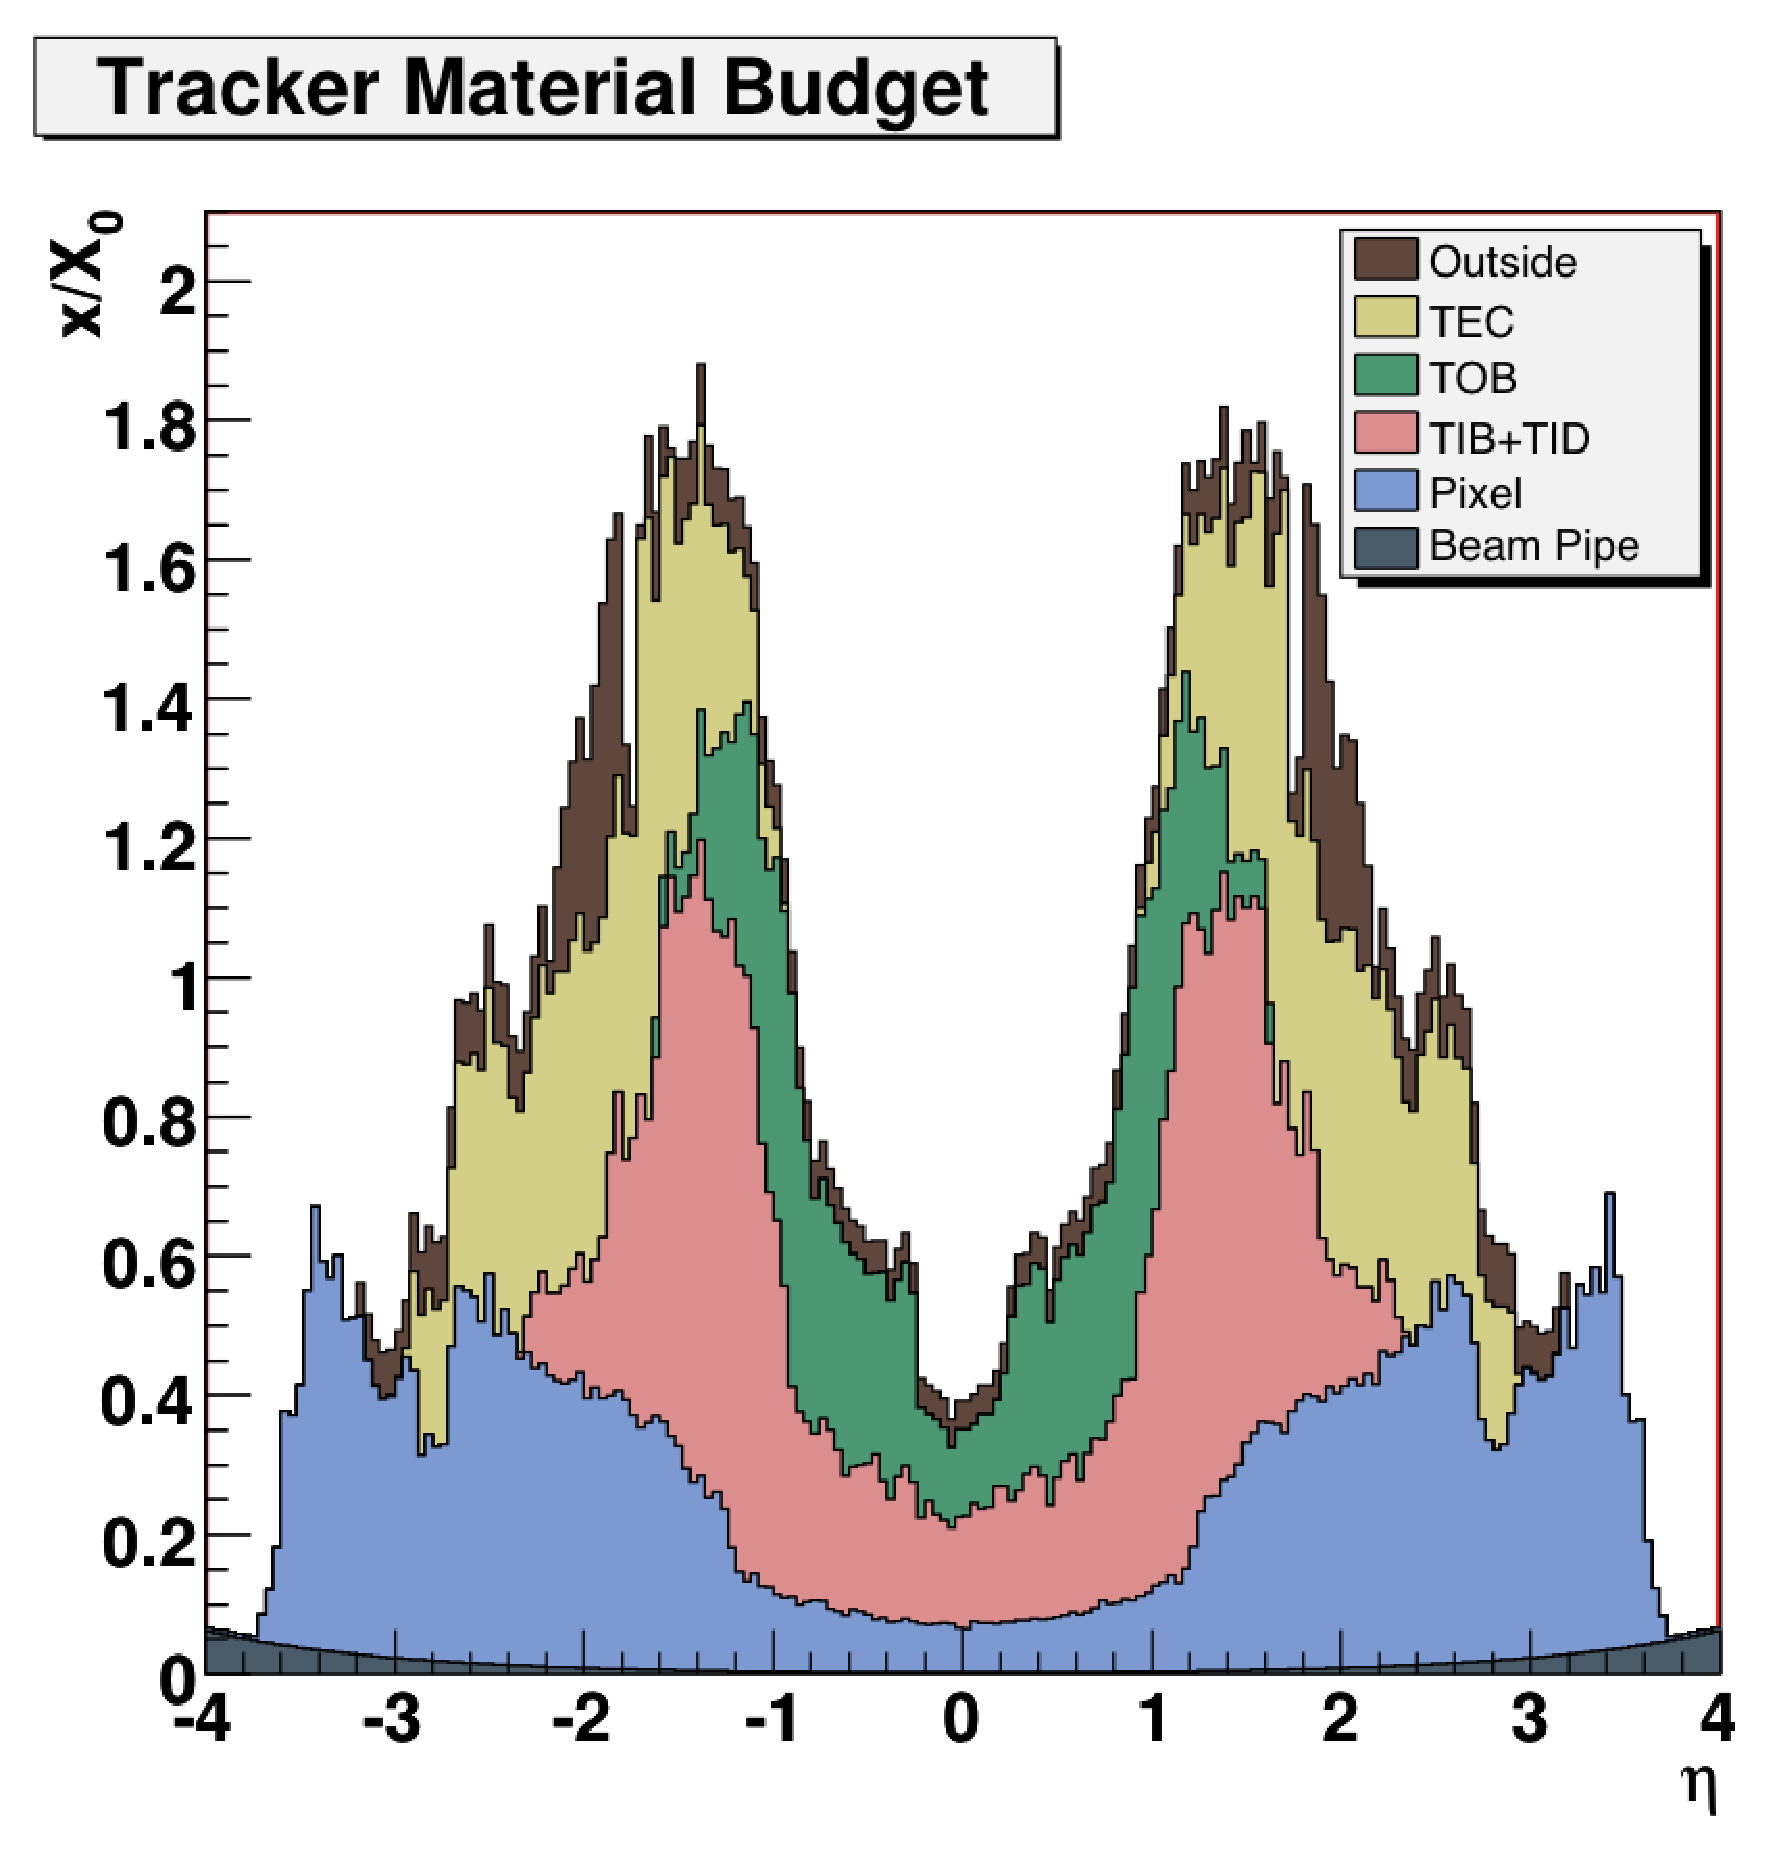
\includegraphics[width=0.4\textwidth]{material.pdf}
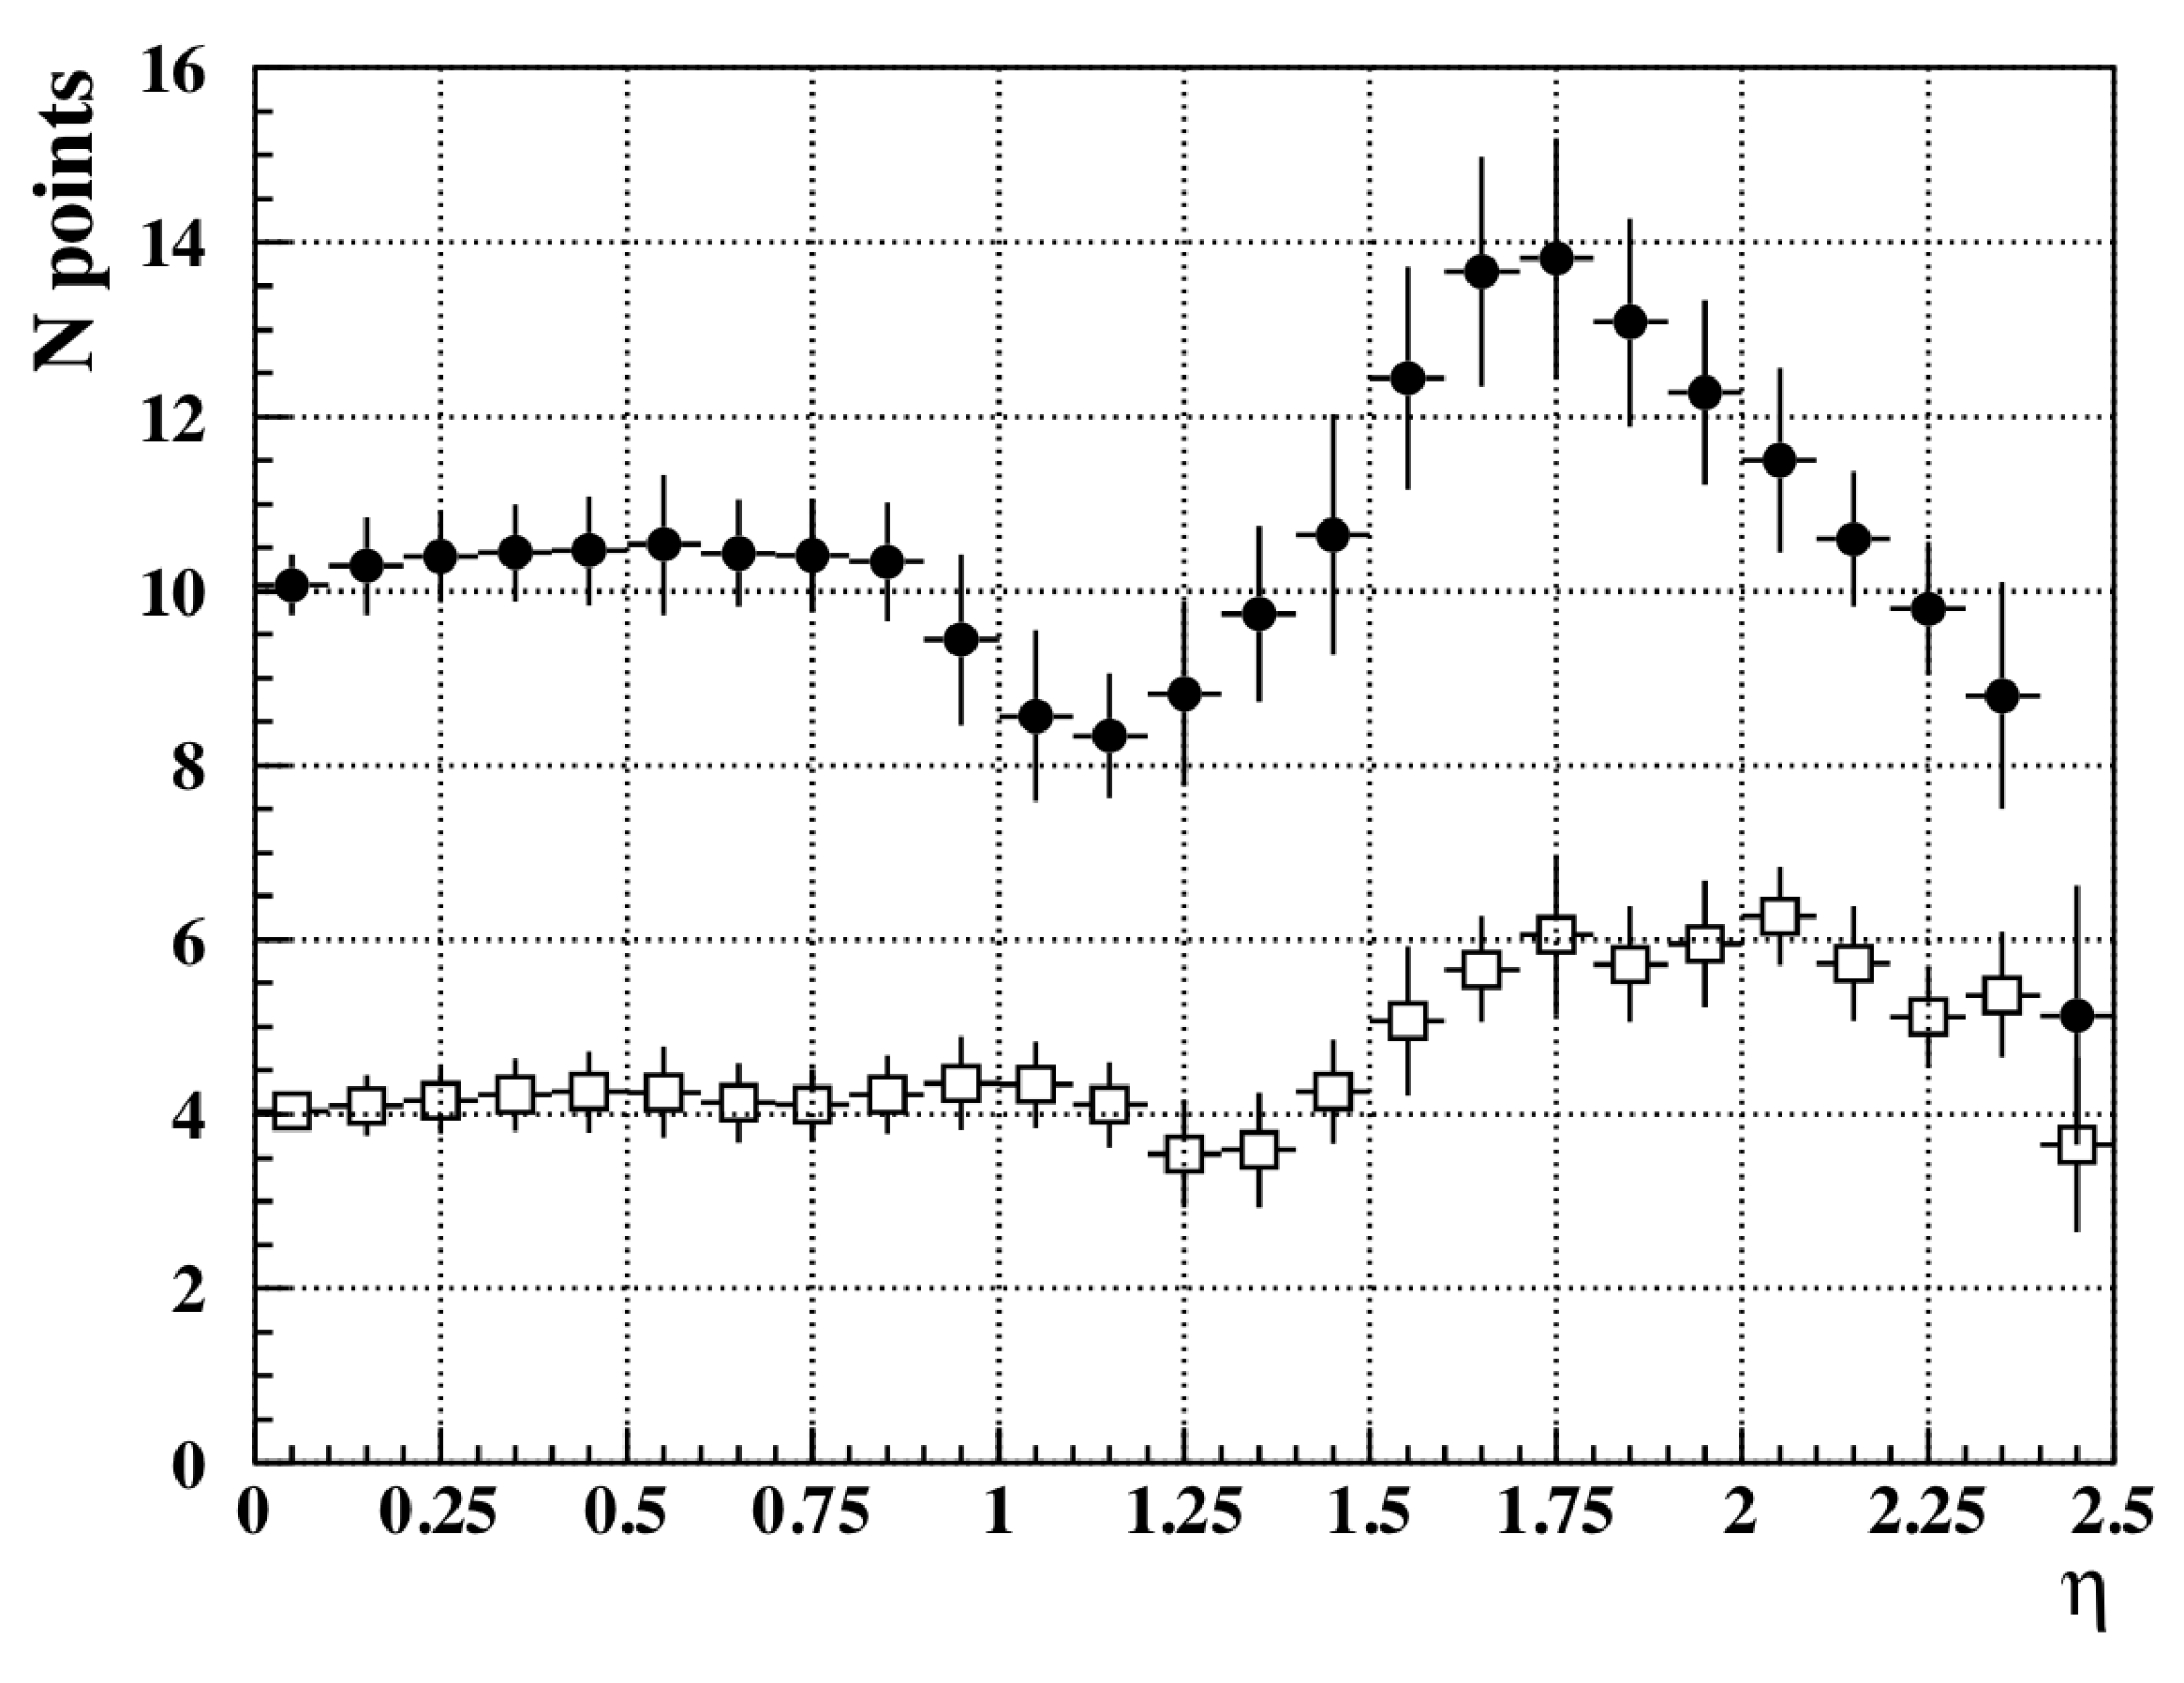
\includegraphics[width=0.55\textwidth]{nhits.pdf}
\caption[
Radiation length and number of layers crossed in the CMS tracker as a function
of pseudorapidity.
]{ \label{fig:cms_material}
Radiation length of the CMS tracker as a function of pseudorapidity
(left). Number of layers passed as a function of
pseudorapidity (right). Black circles represent total layers while hollow
squares represent the number of layers with a stereo measurement~\cite{trackingperformance}.
}
\end{center}
\end{figure}
% --------------------------------------------------------------------------- %

The tracker provides at least ten particle position measurement for any
possible particle trajectory within the tracker's acceptance region
which is about $\aeta < 2.5$. Figure~\ref{fig:cms_material} shows the
number of measurements as a function of $\aeta$. Some of the tracker's
silicon layers have duel layers with a slight offset to facilite a more
accurate positional measured. The number of these stereo layers are also
shown in Figure~\ref{fig:cms_material}. The overall initial transverse
position (traverse impact parameter, \dzero) and the momentum resolution
is shown in Figure~\ref{fig:cms_tkres}. The overall charged particle
reconstruction efficiency, calculated using standard tag and probe
techniques (see Section~\ref{sec:eff_tnp}), is on average greater than
99\%~\cite{trackingperformance}.

% --------------------------------------------------------------------------- %
\begin{figure}[!htb]
\begin{center}
\subfloat{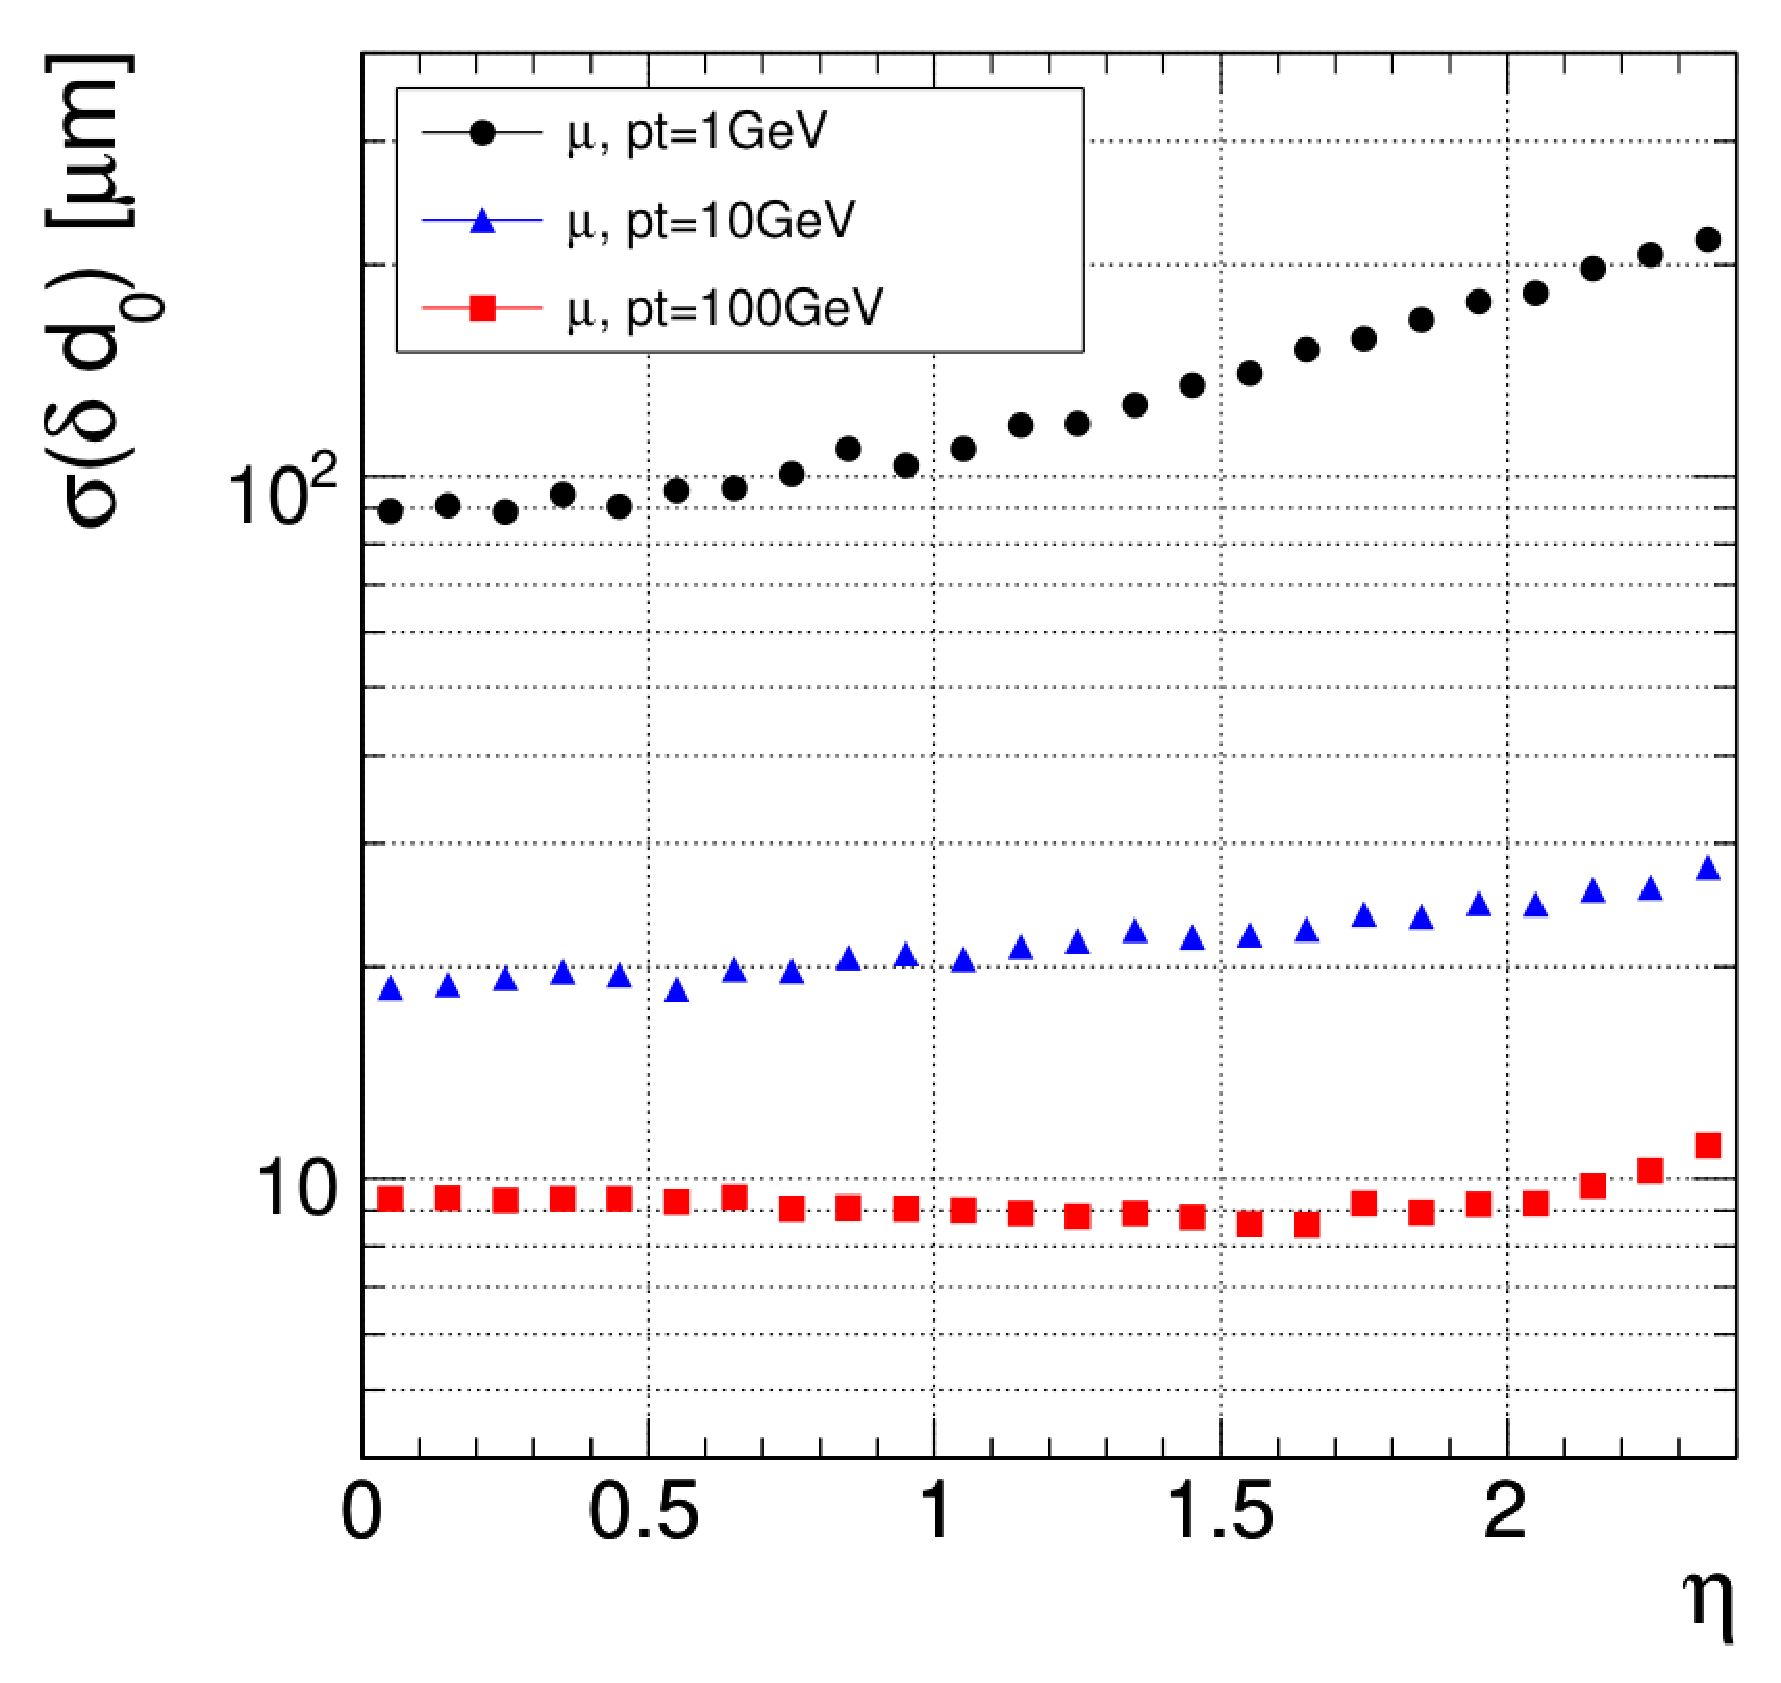
\includegraphics[width=0.45\textwidth]{d0resveta.pdf}} 
\subfloat{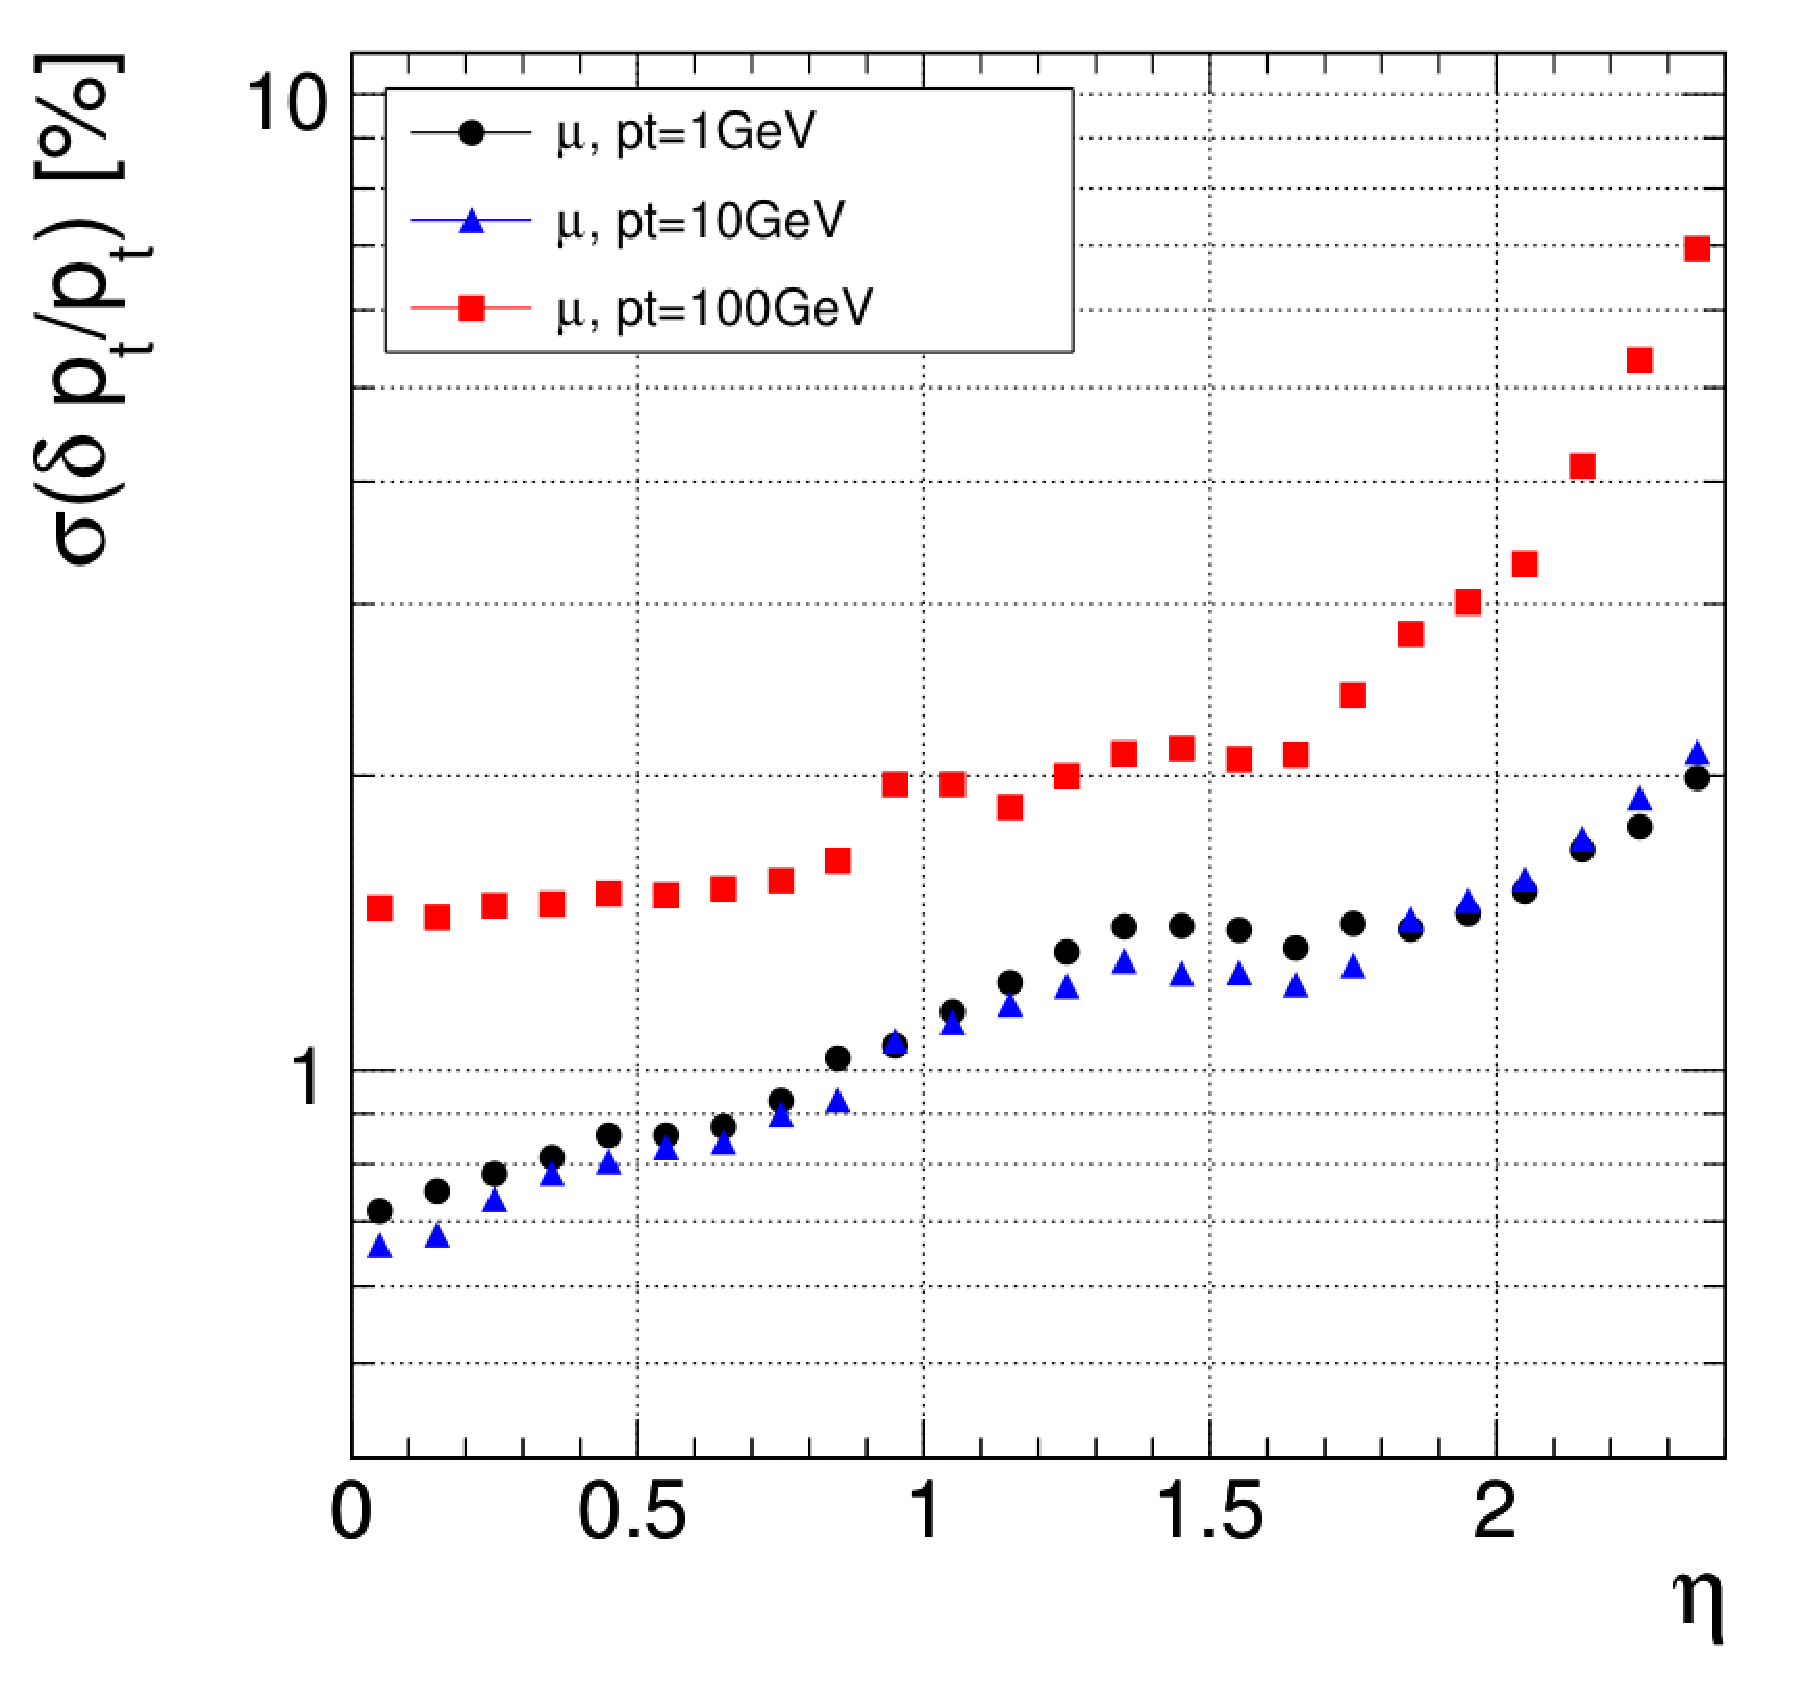
\includegraphics[width=0.45\textwidth]{ptresveta.pdf}}
\caption[
Muon transverse impact parameter resolution and transverse momentum
resolution as a function of pseudorapidity
]{\label{fig:cms_tkres}
Muon transverse impact parameter
resolution (left) and transverse momentum resolution as a function of
pseudorapidity for various muon momenta: 1 \GeV as circles, 10 \GeV as
triangles and 100 \GeV as squares~\cite{trackingperformance}.
}
\end{center}
\end{figure} 
% --------------------------------------------------------------------------- %

% --------------------------------------------------------------------------- %
% --------------------------------------------------------------------------- %
\subsection{The Calorimeters}
\label {sec:cms_calo}
% --------------------------------------------------------------------------- %
% --------------------------------------------------------------------------- %
CMS has two calorimetry detectors, both situated inside the solenoid. The
first, directly behind the silicon tracker, is the electromagnetic calorimeter
(ECAL), designed to measure the energy of particles which interact primarily
electromagnetically, i.e. electrons and photons. The second, directly behind
the ECAL, is the hadronic calorimeter (HCAL), designed to measure particles
interacting predominately by the strong interaction. Both sub-detectors were
designed to be fully hermetic, have good energy resolution over a large
area of the detector, and hence be able to accurately reconstruct the total
amount of energy released for each proton-proton interaction. Combined, the
calorimeters allow for the detection of neutrinos escaping from the CMS
detector by measuring an energy imbalance in the transverse plane. In addition,
the calorimeters are designed to be thick enough to prevent most particles
from pushing through the solenoid and into the muon chambers. To achieve these
features, both detectors had to be composed of dense and highly segmented
material.

\subsubsection{Electromagnetic Calorimeter}
\label {sec:cms_ecal}

Lead Tungstate (\pbw) crystals were chosen to comprise the fully hermetic and
homogeneous ECAL. \pbw satisfies the needs imposed by the LHC environment: the
radiation resistance allows for long lifetime and the high density satisfies
the space constraints as well as allows for fine granularity and quick read
out times. The homogeneity of the detector allows for good overall energy
resolution. \pbw has a radiation length ($X_0$) of 0.89 \cm and a Moli\`ere
radius of 2.2 \cm. The Moli\`ere radius is a measure of the spread of energy
from showering electrons and photons and is defined as the radius which
contains 90\% of the showering energy. Having a small Moli\`ere radius also
allows for the use of smaller crystals and hence gives higher segmentation.
Finally, \pbw has a quick scintillation decay time which allows for read out
times fast enough to deal with the signed 25 ns interaction spacing of the LHC.

The ECAL barrel (EB) contains 61,200 \pbw crystals arranged in a cylindrical
formation around the silicon tracker. Each crystal is rectangular in shape, 240
mm long ($\sim 26 X_0$), $22 \times 22$ $\rm{mm^2}$ on the front surface and
$26 \times 26$ $\rm{mm^2}$ on the near surface. The EB cover a pseudorapidity
range $\aeta < 1.479$ with each crystal having a size in $\eta - \phi$ space of
$0.0174 \times 0.0174$.

The ECAL endcaps (EE+ and EE-) each contain 7,324 \pbw crystals and cover
pseudorapidity range of $1.479 < \aeta < 3.0$. Each EE is split into an upper
and lower disk, ``dees'' which arrange the crystals in an $x - y$ pattern while
situating the crystal face to point in the direction of the nominal interaction
point. The crystals are approximately $30 \times 30$ mm on their face with a
length of 220 $\rm{mm^2}$ ($\sim 25 X_0$).

In addition to the EB and EE, there is an additional electromagnetic calorimeter
stationed on each side directly in front of the EE. Called the preshower (ES),
this sub-detector gives additional radiation lengths and helps differentiate
electrons and photons from pions. A full schematic of the ECAL system can be
seen in Figure~\ref{fig:cms_ecal}.

% --------------------------------------------------------------------------- %
\begin{figure}[!htb]
\begin{center}
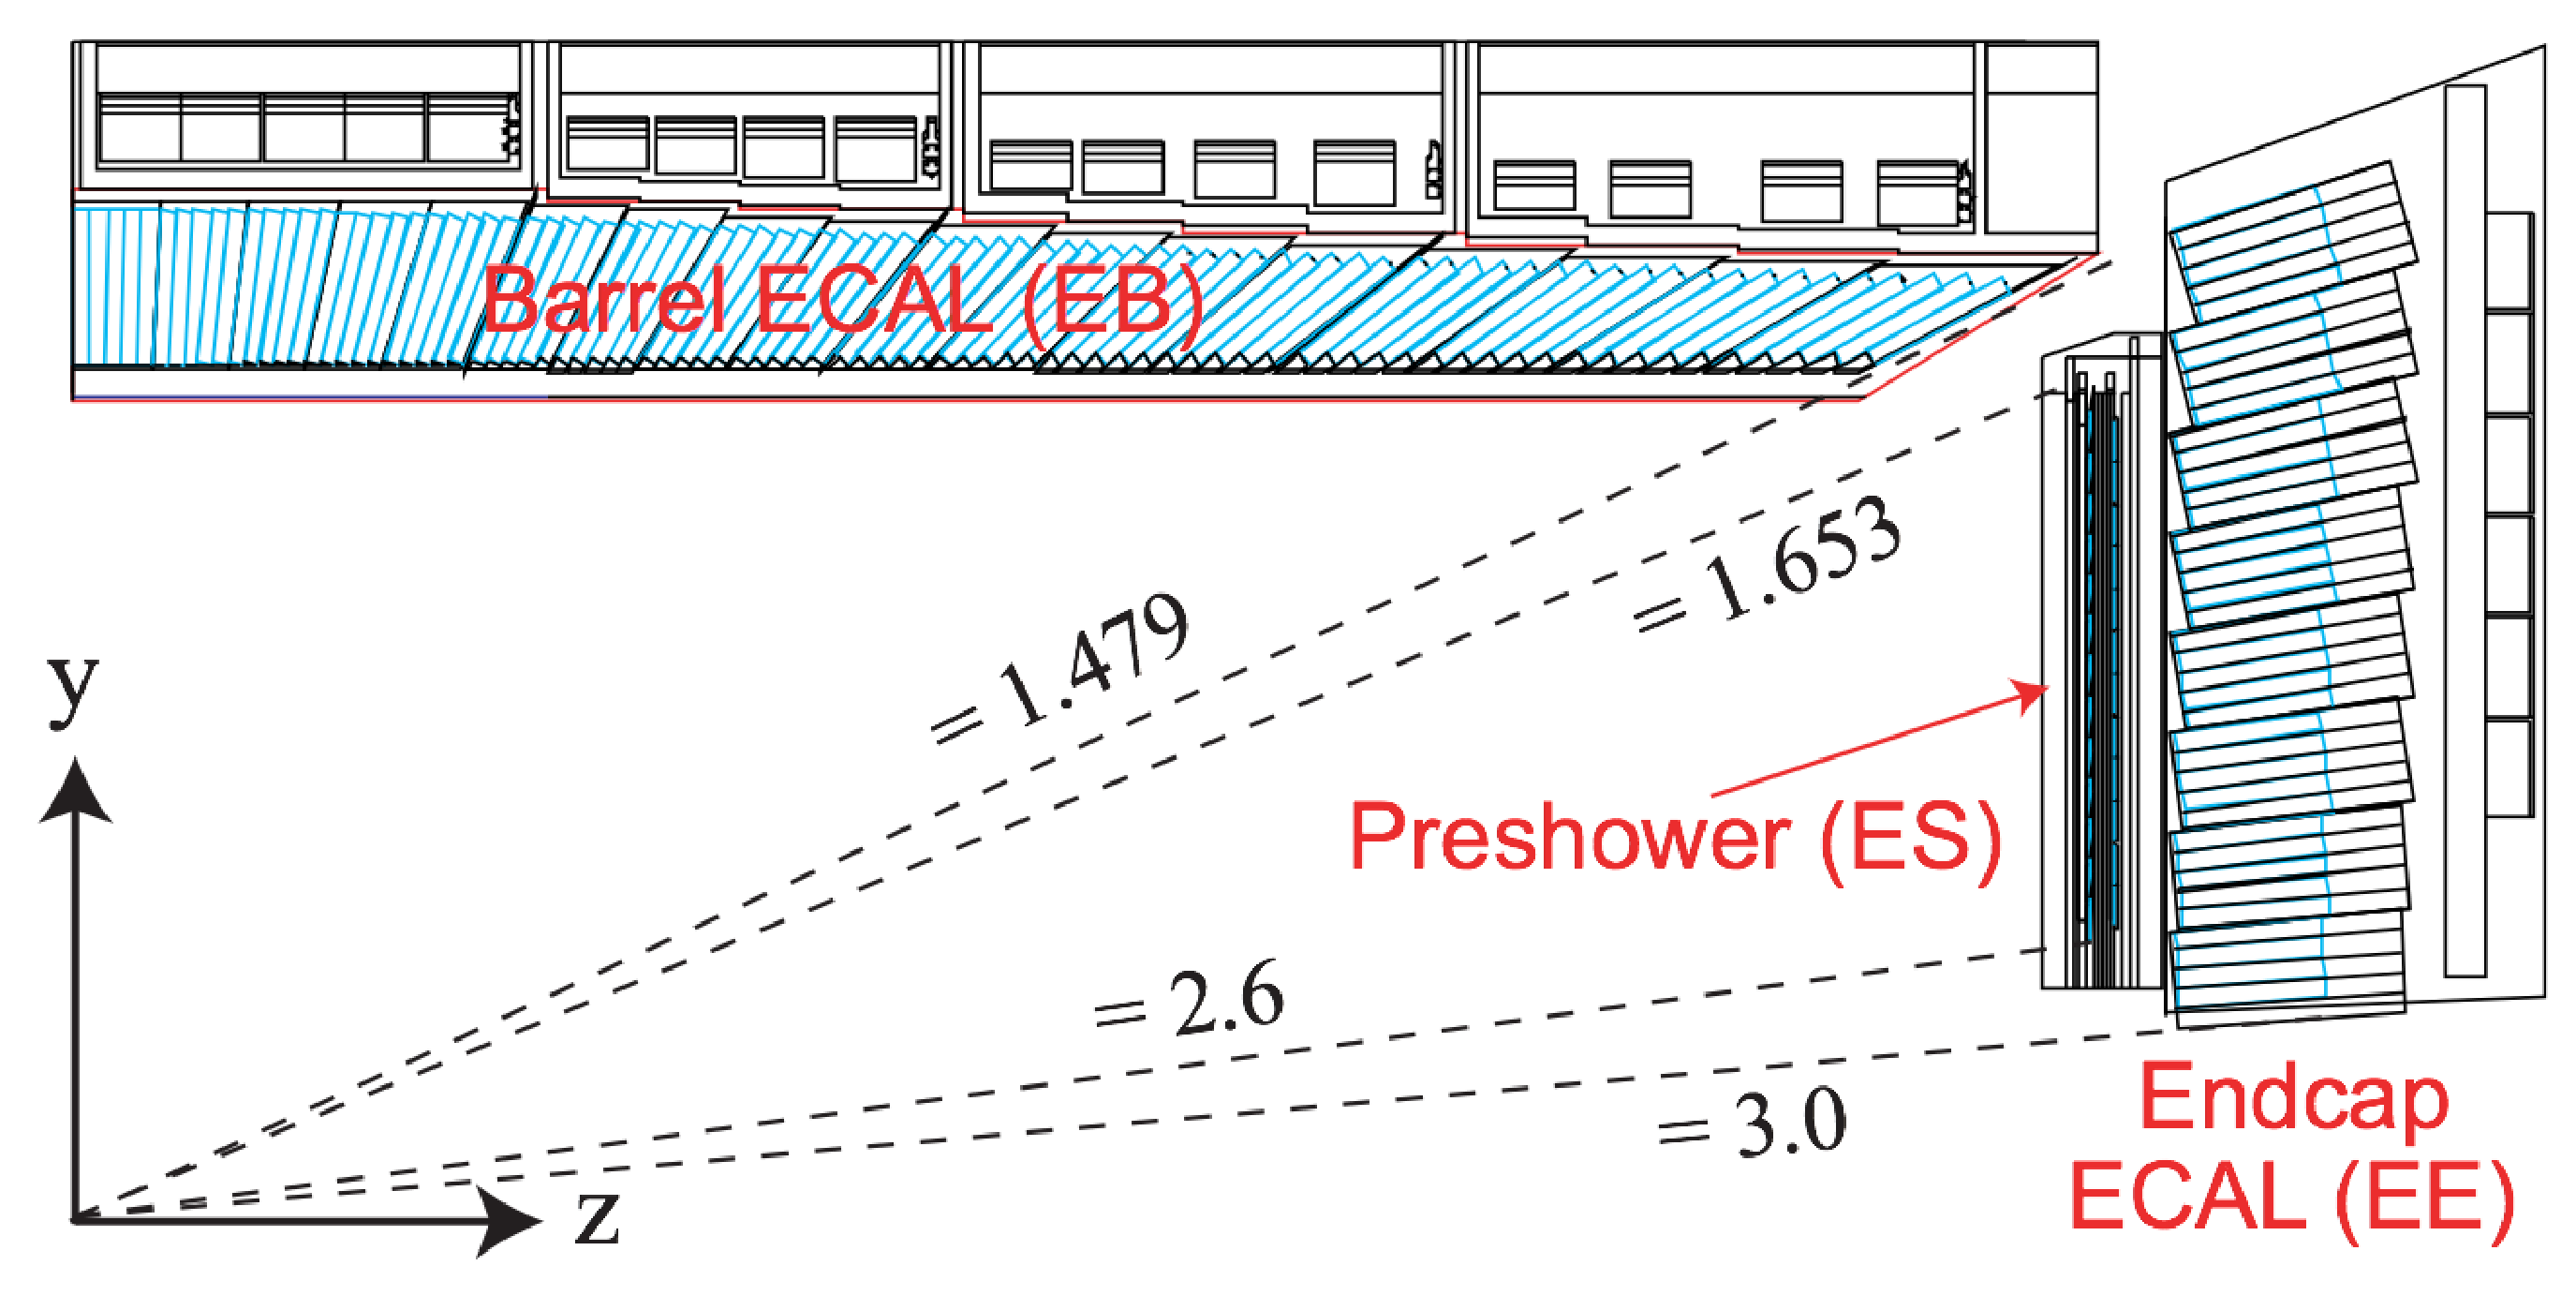
\includegraphics[width=0.8\textwidth]{ecal.pdf}
\caption{\label{fig:cms_ecal}
One quarter of the electromagnetic calorimeter system projected into the $y-z$
plane~\cite{tdr1}.
}
\end{center}
\end{figure}
% --------------------------------------------------------------------------- %

To convert the light created in the crystals to an electrical signal, silicon
avalanche diodes (APDs) and vacuum phototriodes (VPDs) are used in the barrel
and endcap, respectively. Both photo-detectors were designed to be fast, have a
high radiation tolerance and be able to operate in the presence of CMS's strong
magnetic field. In addition, the photo-detectors have to be able to withstand
the bombardment of hadronic particles passing through their active area without
too much disruption and to be able to amplify the low light output of the \pbw
crystals.

\subsubsection{Hadronic Calorimeter}
\label {sec:cms_hcal}

The HCAL sits between the ECAL and the solenoid and is important for the
identification and reconstruction of hadronic energy~\cite{hcalperformance}.
The HCAL is comprised of four different sets of sub-detectors, the HCAL barrel
(HB), the HCAL endcaps (HE), the outer HCAL (HO), and the forward HCAL (HF). A
full schematic of the HCAL system can be seen in Figure~\ref{fig:cms_hcal}.

% --------------------------------------------------------------------------- %
\begin{figure}[!htb]
\begin{center}
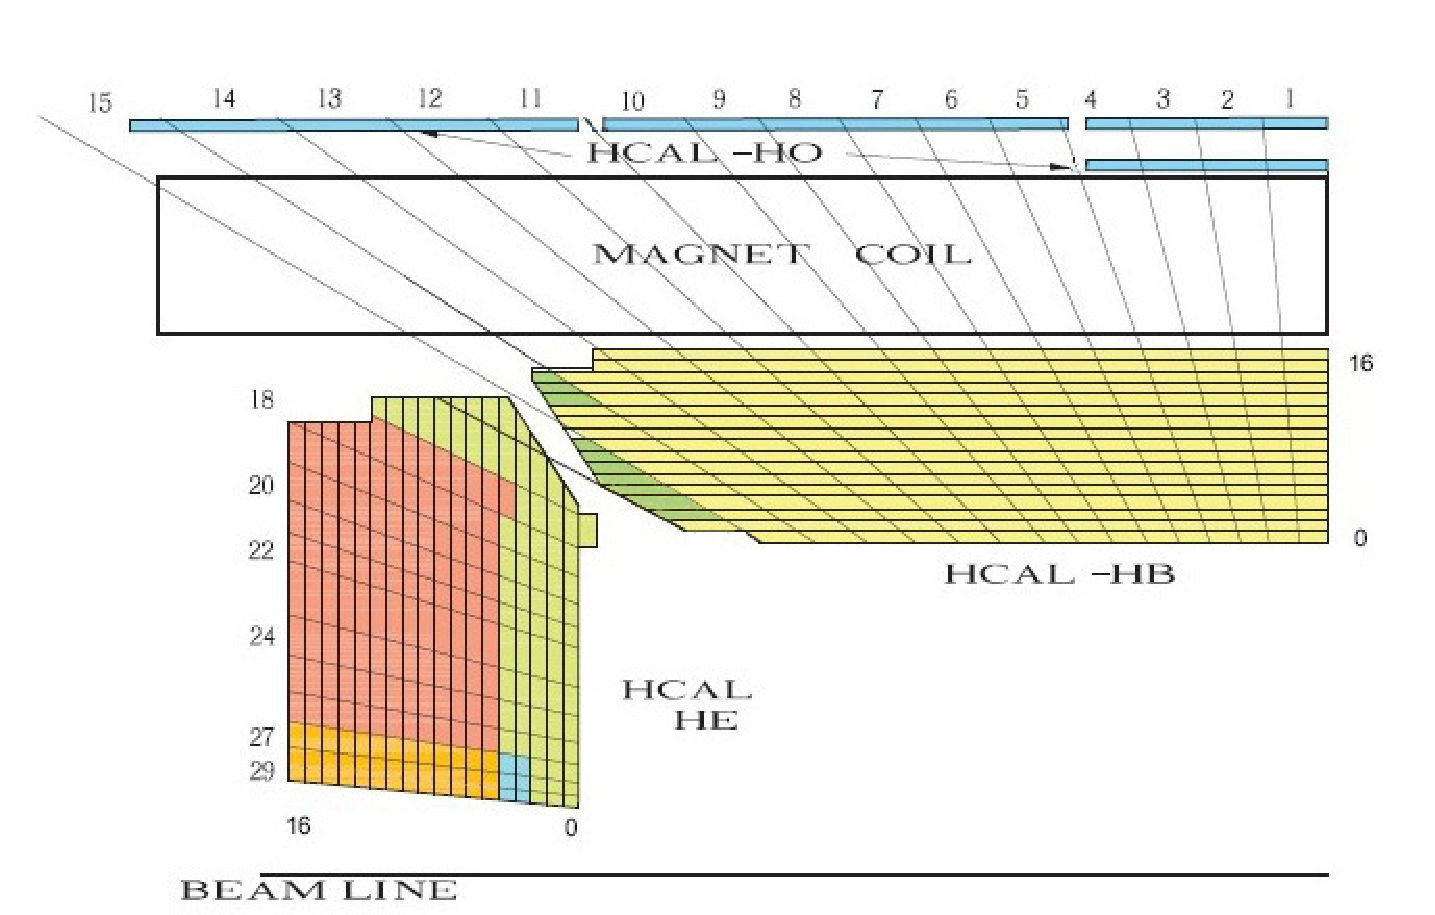
\includegraphics[width=0.9\textwidth]{hcal.pdf}
\caption{\label{fig:cms_hcal}
One quarter of the hadronic calorimeter system projected into the $y-z$
plane~\cite{hcalperformance}.
}
\end{center}
\end{figure}
% --------------------------------------------------------------------------- %

The HB and HE both use brass alloy (70\% Cu, 30\% Zn), which has an interaction
length ($\lambda_I$) of 15 \cm. This ensures as much hadronic showering as
possible while still falling within the spatial and monetary constraints. The
HB covers the \pr range of $\aeta < 1.3$ and contains 36 wedge shaped blocks of
material (18 around the cylinder and each half of the HB). Each wedge consists
of a flat brass absorber plate that runs parallel to the beam axis with plastic
scintillators interspersed throughout, which convert the hadronizing energy
into light for detection. The scintillators are distributed to give a spacial
segmentation of $0.087 \times 0.087$ in $\eta - \phi$ space. The interaction
length of the HB varies from 5.92 to 10.6 $\lambda_I$, depending on the \pr.
The HE takes over where the HB leaves off and covers a \pr range of $1.3 <
\aeta < 3.0$. The granularity in this region allows for positional measurements
with a size of $0.087 \times 0.087$ up to $\eta < 1.6$ and $0.17 \times 0.17$
beyond $\aeta > 1.6$. The total depth of the HE is nine interaction lengths.
Both the HB and HE utilize multipixel hybrid photodiodes (HPD), which operate
well in strong magnetic fields, to convert the scintillator light to an
electric signal.

Between $3.0 < \aeta < 5.0$ sits the HF which, instead of brass, uses steel to
absorb the hadronic particles. Due to the very large particle fluxes in this
region, scintillators were replaced by more radiation hard quartz fibers.
These quartz fibers emit Cherenkov radiation which is then channeled to the
readout photodiodes. The segmentation of the HF gives the approximate size
of each readout channel as $0.18 \times 0.18$ in $\eta - \phi$ space.

Finally, to supplement the energy measurement in the barrel, the region with
the lowest interaction length, the HO sits outside the solenoid. In fact,
it uses the solenoid as an extra absorber material, which gives at least
1.5 interaction lengths, depending on the \pr. The HO utilizes scintillator
material directly behind the solenoid to measure the energy of any particle
which hadronizes inside the solenoid. With the ECAL giving approximately one
interaction length, the total interaction length of CMS is always greater
than 11.8, giving $< 0.1\%$ chance of a hadron punching through to the muon
detectors.

% --------------------------------------------------------------------------- %
% --------------------------------------------------------------------------- %
\subsection{The Muon Detectors}
\label {sec:cms_musys}
% --------------------------------------------------------------------------- %
% --------------------------------------------------------------------------- %
The Compact Muon Solenoid was designed to efficiently and precisely detect
muons. Muons, unlike the much lighter and radiative electrons, interact very
minimally with matter, traversing even the densest parts of CMS (the ECAL and
HCAL) with relative ease while at the same time depositing very little of its
energy. Muons are also relatively long lived and their lifetime allows them to
be measured by the CMS detector before it decays. It is for these reasons that
the muon detectors are situated outside the solenoid, far from the interaction
point.

The muon system employs three different gas-based particle detectors which
allow for excellent muon measuring capabilities. In addition to positional
measurements, the muon detectors also provide muon identification, momentum
and triggering (see Section~\ref{sec:cms_daq}). The chambers sit inside CMS's
iron return yoke which acts as an absorbing material for hadrons and other
non-muon particles which try to penetrate through the solenoid. In the barrel,
the drift tube (DT) sub-detector sits cylindrically concentric. The endcap
houses cathode strip chambers (CSC) which consist of four layers on each side
of the barrel. Finally, interspersed through the barrel and endcap, is the
resistive plate chambers (RPC) used to enhance the timing resolution of the
detection of muons. A graphical overview of the CMS muon system is shown in
Figure~\ref{fig:cms_musys}.

% --------------------------------------------------------------------------- %
\begin{figure}[!hbt]
\begin{center}
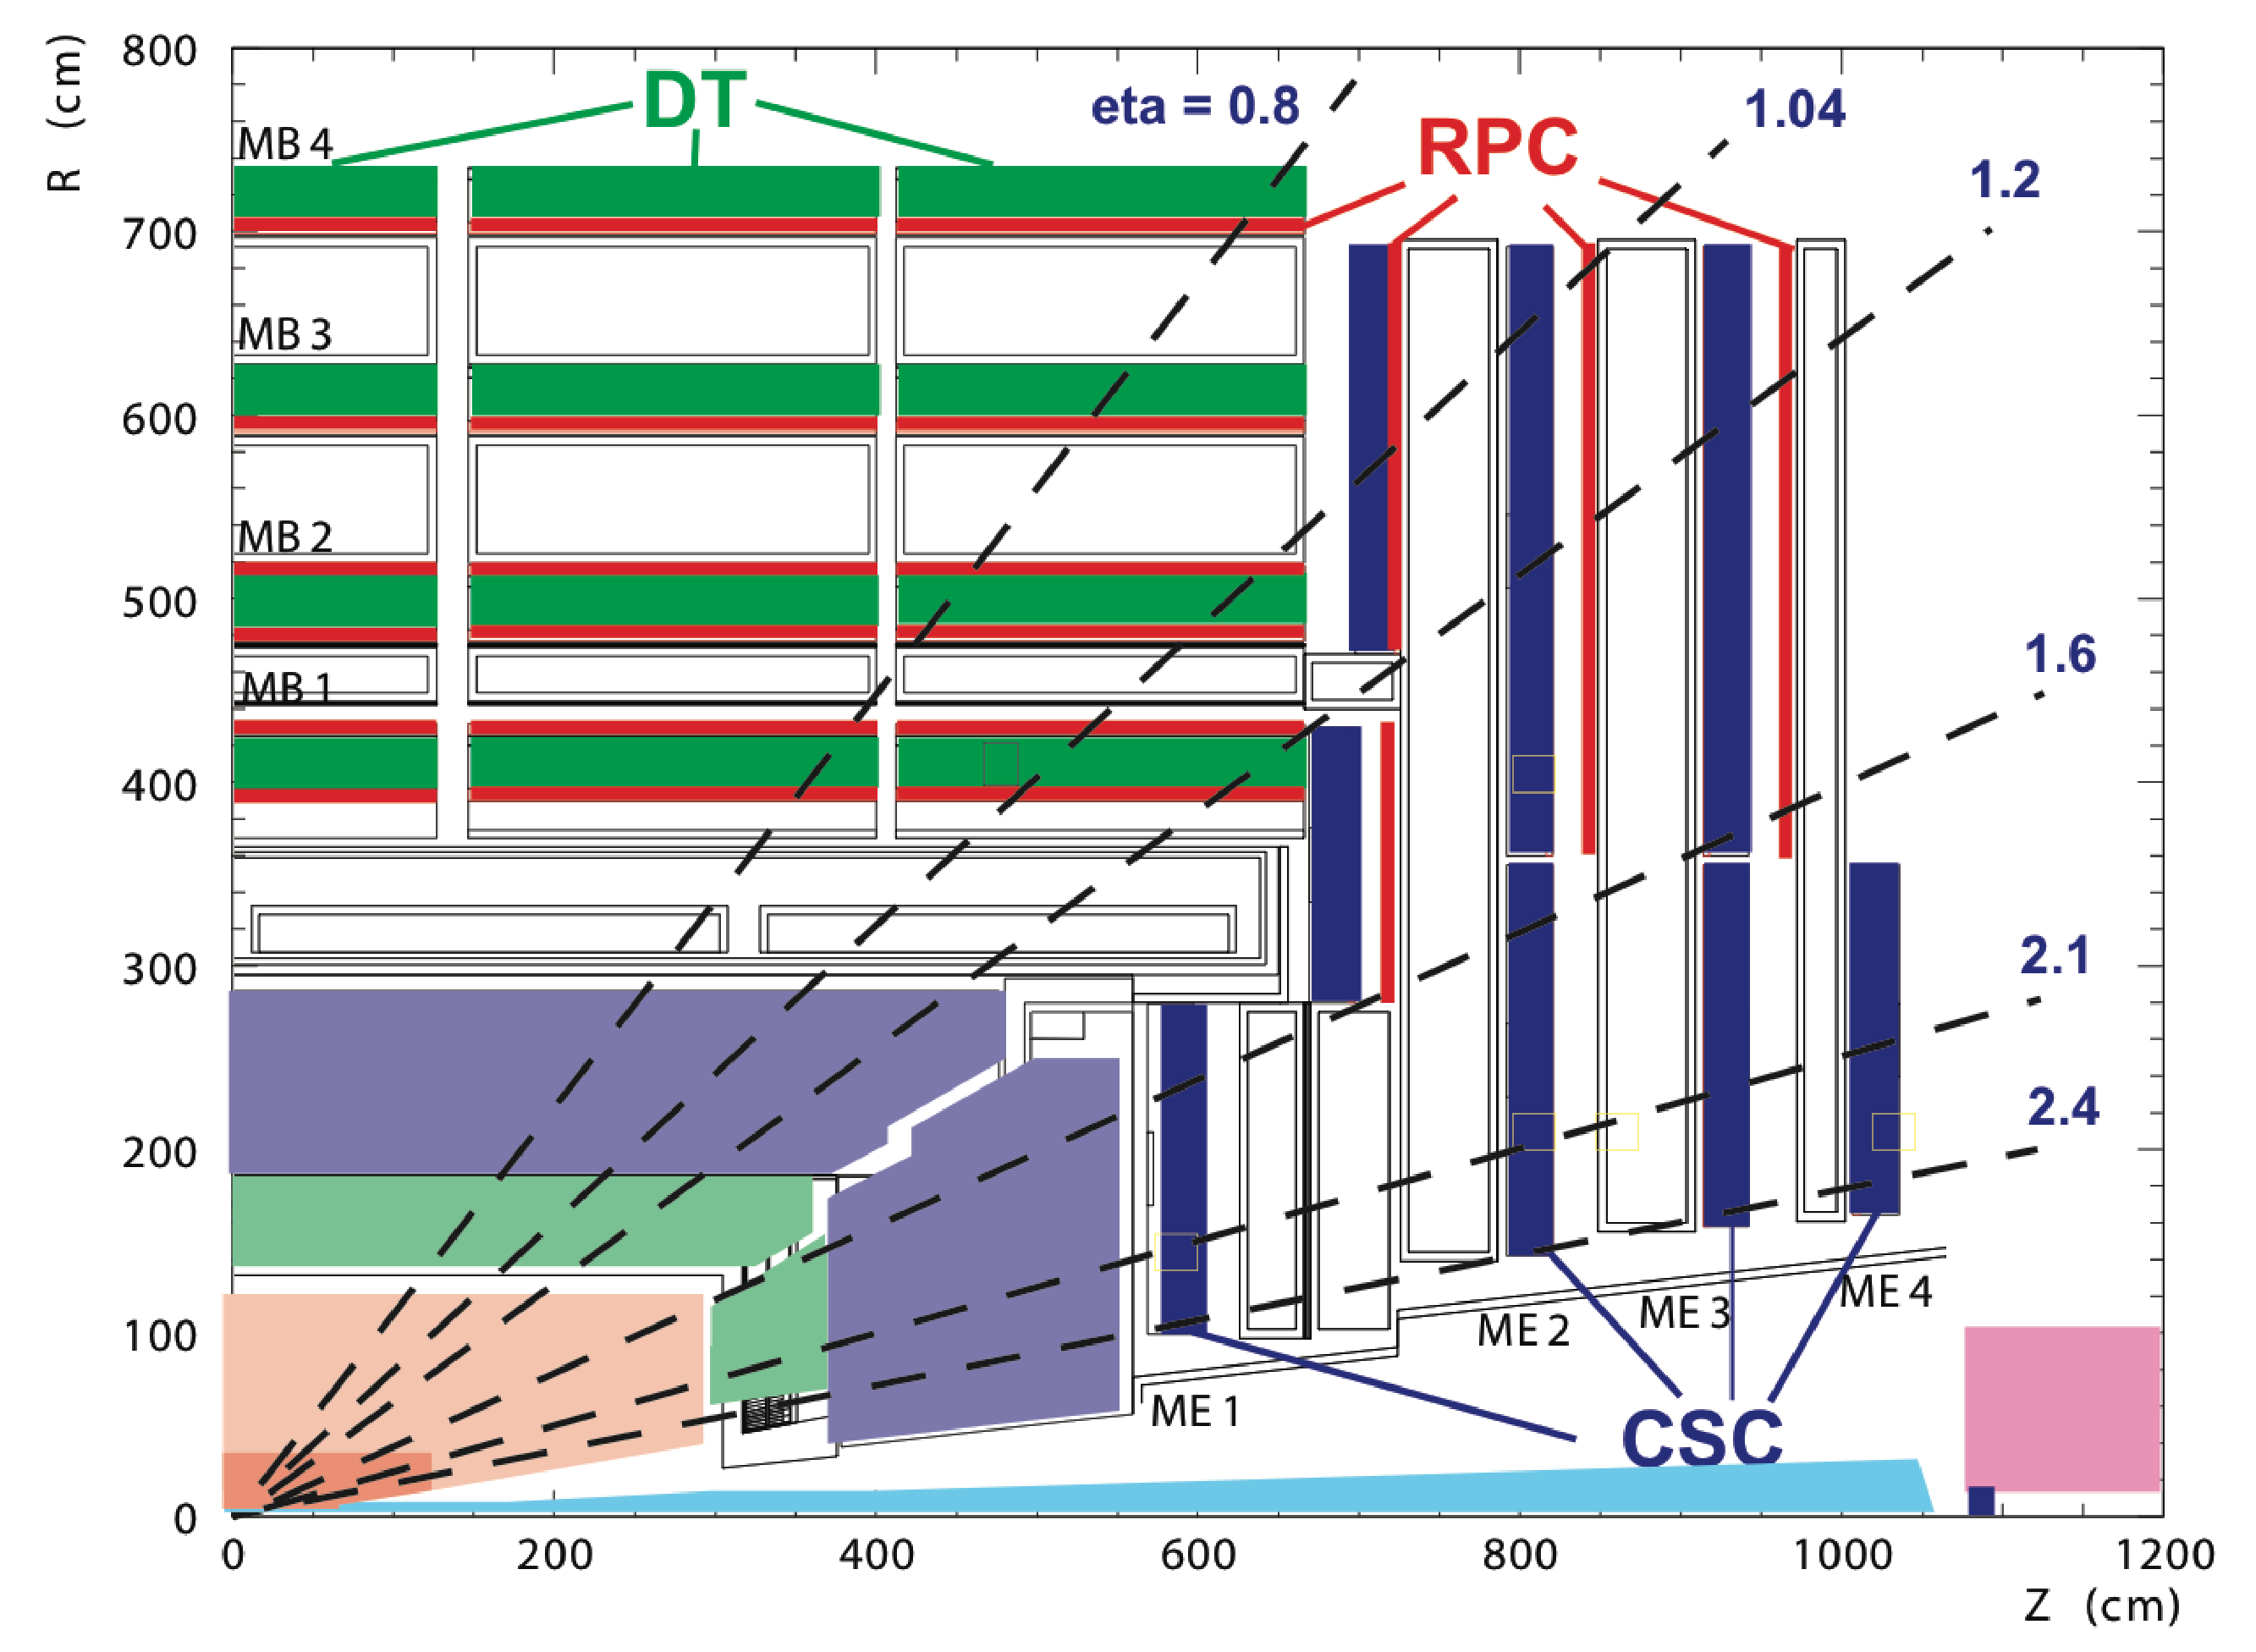
\includegraphics[width=0.8\textwidth]{musys.pdf}
\caption[Overview of the CMS muon subdetector system]
{\label{fig:cms_musys}
Overview of the CMS muon sub-detector system. The drift tubes, situated in the
barrel region, are shown in green, the cathode strip chambers, situated in the
endcap region, are shown in blue and the resistive plate chambers, situated
throughout, are shown in red~\cite{muontdr}.
}
\end{center}
\end{figure}
% --------------------------------------------------------------------------- %

\subsubsection{Drift Tubes}
\label {sec:cms_musys_dt}

Drift tubes are long cylindrical tubes filled with gas and threaded with an
equally long conductive wire (the anode). The inside of the cylinder is also
lined with a conductive material (the cathode). The gas, a mixture of noble gas
with full set of valence electrons, relinquishes electrons as charged particles
traverse through it. A bias voltage is applied across the wire and the cylinder
causing the electrons to flow one way and particle detection is achieved through
measuring the amount of induced current.

The DT system sits in the barrel region outside the solenoid and
covers a \pr range $\aeta < 1.2$. Each set of drift tubes are arranged as a
rectangular chamber and staggered throughout the return yoke. There are 250
chambers arranged in four concentric cylinders of chambers (stations) divided
by five rings (wheels) of the return yoke. The chambers have a slight overlap
to ensure the hermeticity in 12 different sectors of each ring and wheel, each
covering $30^{\circ}$ in azimuthal angle. The four stations and two and a half
of the wheels can be seen in green in Figure~\ref{fig:cms_musys}.

Each chamber except the last has three sets (superlayers) of four planes
of drift tubes. Tow of the superlayers in each chamber run parallel to the
beam direction to measure the $r-\phi$ position. The third superlayer in the
first three chambers have drift tubes that run perpendicular to the beam line
allowing an additional measurement in the z-direction.

In all, there are over 172,000 drift tubes in the DT system each with an
approximate length of 2.5 m. This length, coupled with the low background and
muon rates and the uniform magnetic field in this region of the detector allow
for the one-dimensional position measurements of the DT system. The DT's give a
time resolution of $\sim$25 ns, well within the timing constraints of the LHC,
and a global resolution in the $r-\phi$ direction of 100 \um.

\subsubsection{Cathode Strip Chambers}
\label {sec:cms_musys_csc}

A cathode strip chamber is similar to a drift tube chamber in that it is
a gaseous detector filled with anode wires; however, instead of a wire
tube per cathode tube, the anode wires are stretched in parallel and are
surrounded on either side by a plan of cathode material. One plane of the
cathode is segmented into strips which run perpendicular to the anode wires.
The induced charge distribution on the wires and strips gives a fully
two-dimensional measurement of a passing particle (in addition to the third
known position given by the position of the chamber). In addition to giving a
three-dimensional positional measurements, the CSCs were also designed with a
fast response time, fine segmentation and to be radiation hard in order to deal
with increased background and muon rates and the non-uniform magnetic field in
the endcap region (as opposed to the lower rates in the barrel where positional
ambiguity can be tolerated).

The CSCs operate in the \pr region $0.9 < \aeta < 2.4$. Similar to the
barrel, there are four stations in each endcap region, arranged in radial
disks perpendicular to the beam line. There are 468 chambers in total, each
trapezoidal in shape and arranged side-by-side circularly around the beam line
in two concentric circles. The anode wires run along the azimuthal direction
and provide the radial measurement while the strips run lengthwise in a radial
direction and give a measurement in $\phi$. The overall positional resolution
of the CSC is between 75 and 150 \um. The CSC system is shown in blue in
Figure~\ref{fig:cms_musys}.

\subsubsection{Resistive Plate Chambers}
\label {sec:cms_musys_rpc}

The goal of the RPC muon detector system is to compliment the CSCs and DTs
by adding faster readout times at the expense of position resolution. The
RPC chambers consist of two gaseous regions separated by a common
strip readout anode plane which gives adequate positional resolution.
Operating with a time resolution well below the minimum of 25 ns,
the RPCs are ideal detectors to be used to ``trigger'', the CMS detector
(see Section~\ref{sec:cms_daq}). The RPC system covers a \pr range of
$\aeta < 1.6$. Originally designed to cover the full range, it will be
completed during the next upgrade. The RPC chambers can be seen in red in
Figure~\ref{fig:cms_musys}. Running along the beam direction (and hence
measuring the azimuthal angle), six (three) layers of chambers exist in the
barrel (endcap) with over 480 chambers in total each approximately 2.5 meters
in length.

\subsubsection{Summary}
\label {sec:cms_musys_summary}

Overall, the muon system was designed to have an efficiency of over 95\% for
detecting muons with a resolution of less that 10\% for muons up to $\pt =
200 GeV$, increasing with resolution between 15\% and 40\% for 200 \GeV to 1
\TeV muons (depending on \aeta). Using the tracker as an additional set of
measurements on the muon, the expected resolution improves to around 1\% for
lower \pt muons and down to approximately 5\% for muon in the TeV range. The
expected resolution on the transverse momentum measurement can be seen for two
different \pr ranges in Figure~\ref{fig:cms_mures}.

% --------------------------------------------------------------------------- %
\begin{figure}[tbhp]
\begin{center}
\subfloat{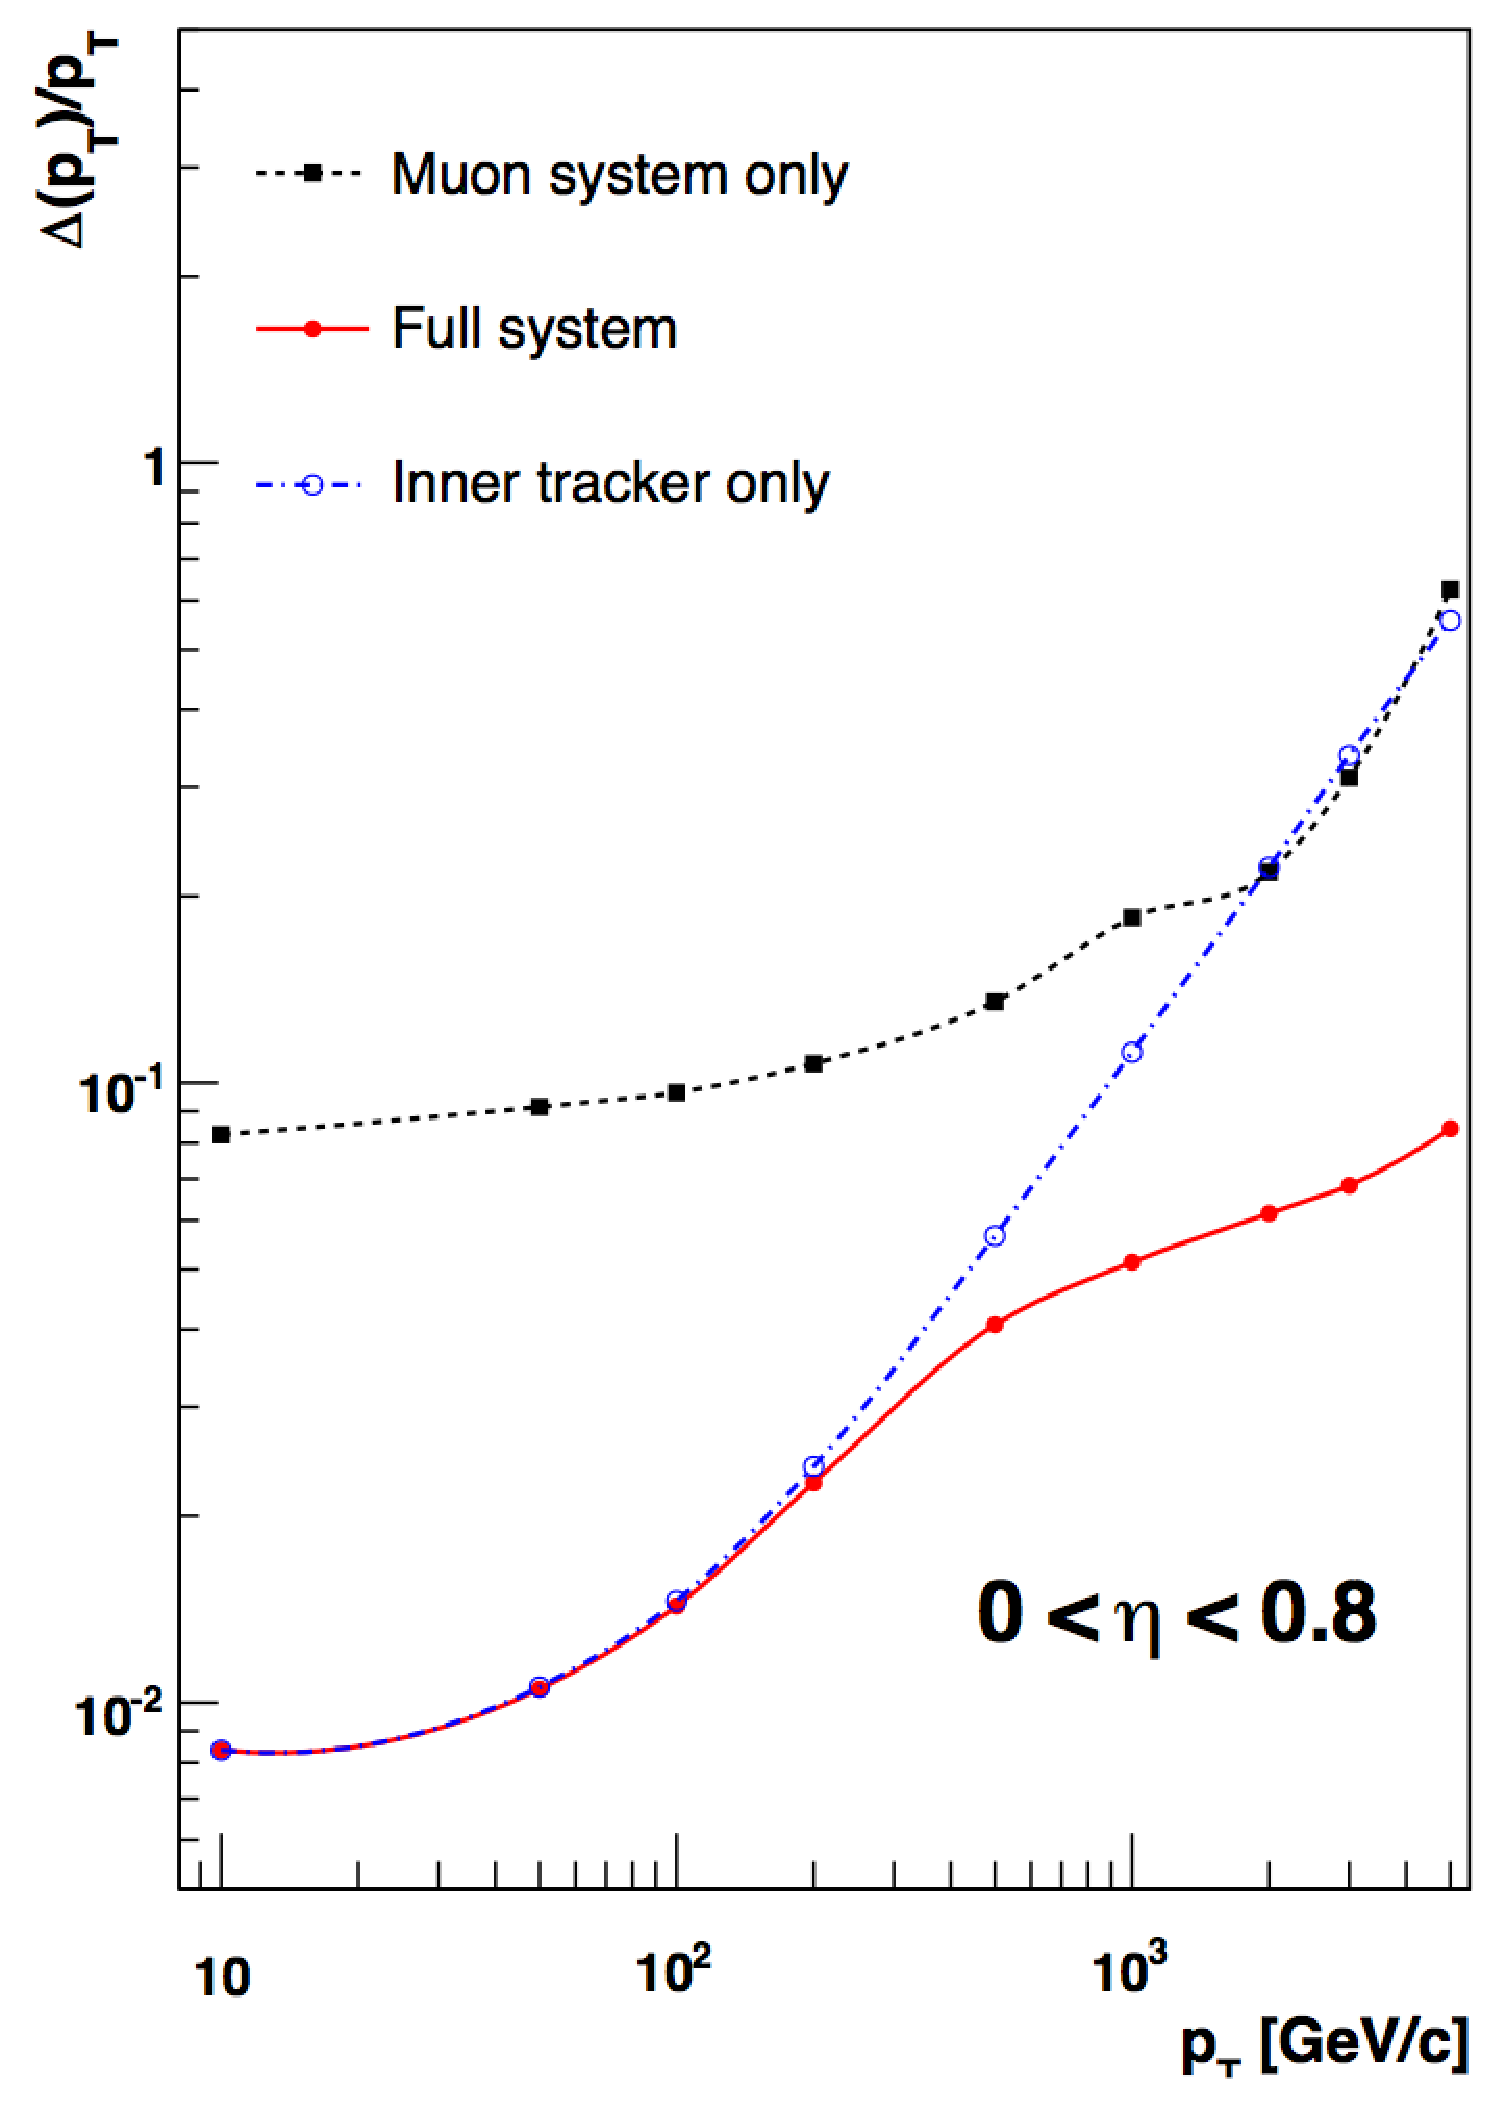
\includegraphics[width=0.40\textwidth]{muresloweta.pdf}} \hspace{5mm}
\subfloat{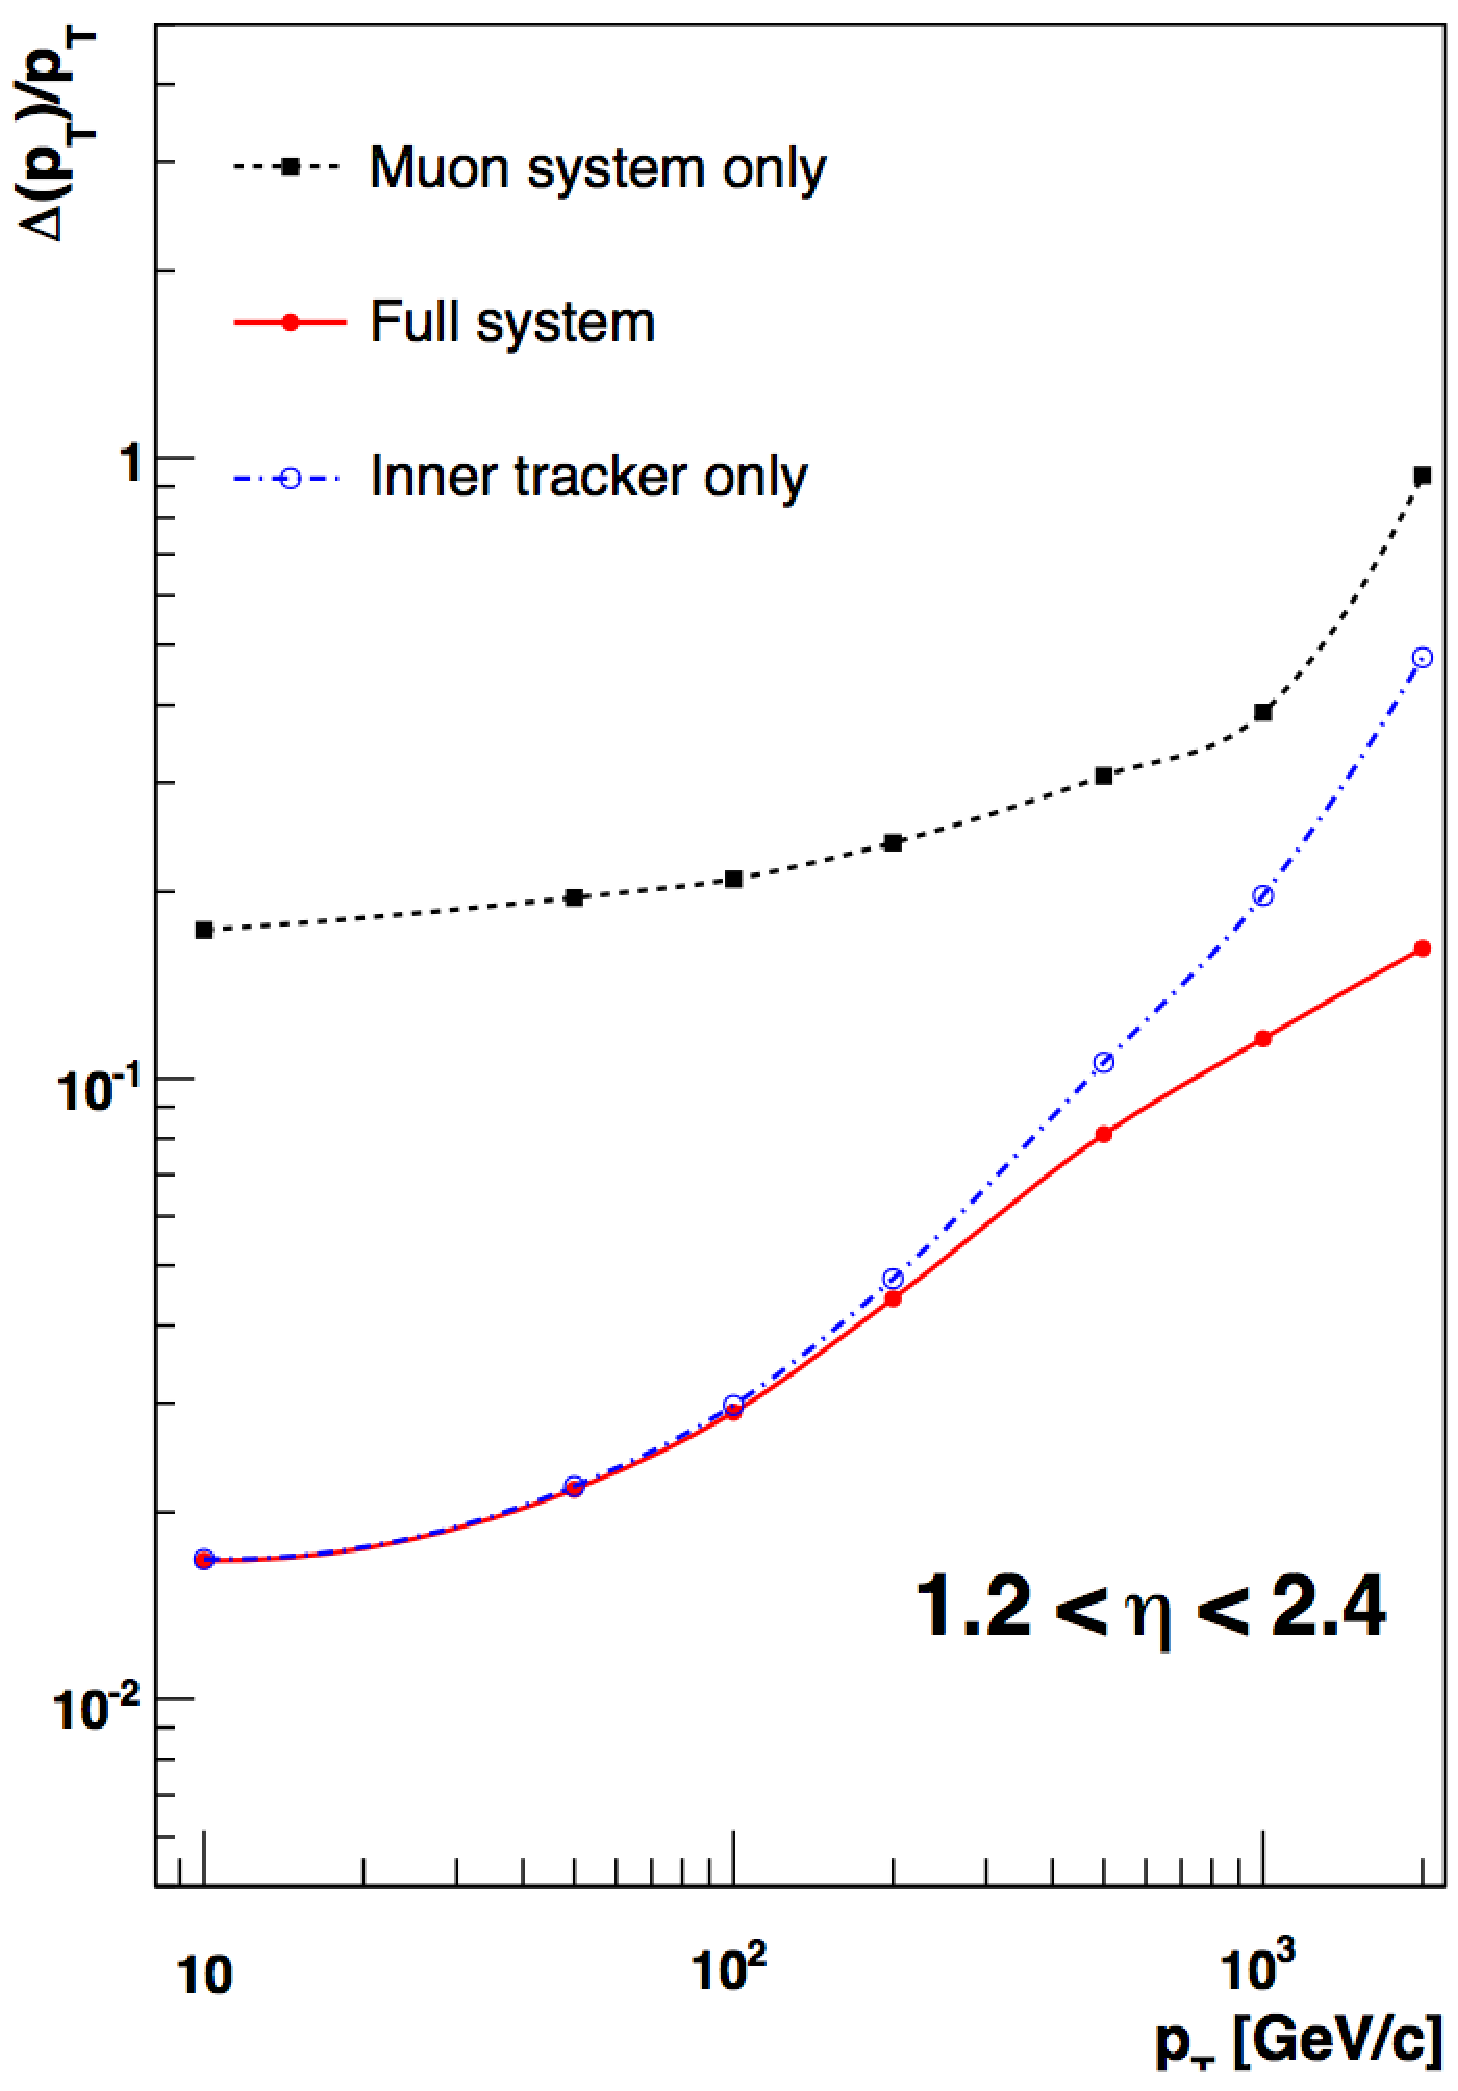
\includegraphics[width=0.39\textwidth]{mureshigheta.pdf}} \\
\caption[Muon momentum resolution for two different pseudorapidity regions]
{\label{fig:cms_mures}
Muon momentum resolution for two different pseudorapidity regions, $0< \aeta
<0.8$ (left) $1.2< \aeta <2.4$ and (right), as a function of transverse
momentum using only the muon system (black), only the inner tracker (blue) and
the combined muon and tracker detectors (red)~\cite{tdr1}.
}
\end{center}
\end{figure} 
% --------------------------------------------------------------------------- %

% --------------------------------------------------------------------------- %
% --------------------------------------------------------------------------- %
\section{Integrated Luminosity Calculation}             \label {sec:cms_lumi}
% --------------------------------------------------------------------------- %
% --------------------------------------------------------------------------- %
CMS uses two different techniques to measure the instantaneous luminosity,
and subsequently the total integrated luminosity~\cite{lumi11, lumi12,
lumi12up}. Both methods employ the use of Van der Meer scans~\cite{vdm},
modulation of the two beam positions until maximum overlap is achieved to
determine the maximum instantaneous luminosity.

The first method uses HF calorimeters which are forward at $\aeta
> 3.0$ and measures the average fraction of empty calorimeter readouts when
triggering on zero-bias events defined by random triggers which are completely
agnostic of activities in the detector. This fraction is converted into a
cross section measurement which can be used to measure the instantaneous
luminosity~\cite{lumi11}.

The non-linear HF response as a function of the instantaneous luminosity, among
other problems, led to the creation and use of the second method~\cite{lumi12,
lumi12up}. This method relies on the fine granularity of the pixel detector.
With a very small fraction ($\sim 0.1\%$) of particles leaving deposits in the
same pixel, the number of pixel clusters during a bunch crossing is found to
be directly related to the proton-proton cross section, which can be related to
the luminosity.

The data used in this analysis was taken over the course of 2012, during which
time the LHC delivered approximately 23.3 \fbinv. Between April and December
of that year, CMS was able to record 21.8 \fbinv of this data of which 19.5
\fbinv was certified by the CMS collaboration as usable for this analysis. The
uncertainty from the luminosity measurement used for all analyses using 2012
data in CMS is 4.4\%. This error must be taken into account for any process
which is estimated from simulation. Figure~\ref{fig:cms_lumi} shows the amount
of data delivered by the LHC and recorded by the CMS detector as a function of
time in 2012.
% --------------------------------------------------------------------------- %
\begin{figure}[!tbh]
\begin{center}
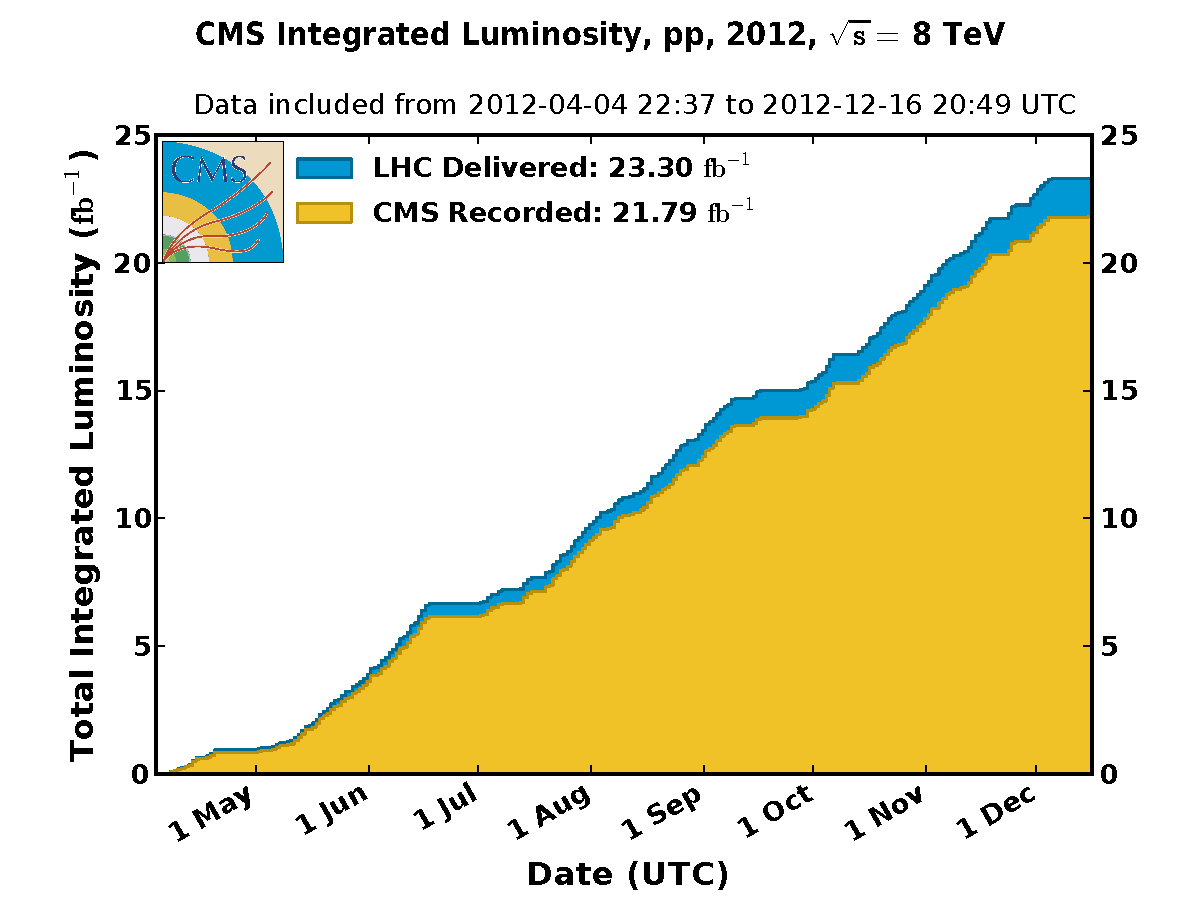
\includegraphics[width=0.8\textwidth]{lumi.pdf}
\caption[Summary of the amount of data delivered by the LHC and collected by CMS in 2012]
{\label{fig:cms_lumi}
The amount of data delivered by the LHC (red) and the amount of data
collected by the CMS detector (blue) as a function of date in the year 2012~\cite{lumitwiki}.
}
\end{center}
\end{figure}
% --------------------------------------------------------------------------- %

% --------------------------------------------------------------------------- %
% --------------------------------------------------------------------------- %
\section{Data Acquisition and Triggering}               \label {sec:cms_daq}
% --------------------------------------------------------------------------- %
% --------------------------------------------------------------------------- %
With nearly 80 million channels, and a bunch crossing every 25 ns having up to
40 proton-proton interactions per crossing, a huge amount of data is produced
by the CMS detector when the LHC is running at or near design luminosity.
At approximately 100 kilobytes of data per interaction, computing design
constraints limit the number of interactions that can be written to disk to
$\sim1000$ per second. The 25 ns between bunches give an interaction rate of 40
MHz resulting in a data reduction requirement of $\sim 10^5$. To accomplish
this, CMS has designed a data acquisition (DAQ) and trigger system which
utilizes a massive computing infrastructure and custom hardware. It is designed
to keep the most interesting interactions across a broad range of physics
goals. If a proton-proton interaction (an event), doesn't pass the trigger
system, it is lost forever.

Triggering occurs in two stages, the first of which is called Level
1 (L1) and has the task of reducing the load from 40 MHz down to 100
kHz~\cite{triggertdr1}. To do so, it employs a farm of custom electronics using
only coarse and lower resolution data to make decisions while storing the rest
of the event data in pipelines awaiting processing. Here, only calorimetric
and muon chamber information is available to make decisions based on the
energy and quantity of depositions in the detector. The data from the events
passing the L1 trigger are processed, compressed and zero-suppressed and sent
for handling by the DAQ. The DAQ then stores and processes the information and
sends it along to the second trigger phase. The High Level Trigger (HLT) is
a farm of standard CPUs running parallel that can run a more complete event
reconstruction to facilitate more informed decisions on whether to keep the
event. The object reconstruction algorithms used are simplified version of the
algorithms described in the following Section. A cartoon representation of the
trigger and DAQ chain can be seen in Figure~\ref{fig:cms_daq}. Between these
two trigger systems, the desired data reduction is achieved.

% --------------------------------------------------------------------------- %
\begin{figure}[tbhp]
\begin{center}
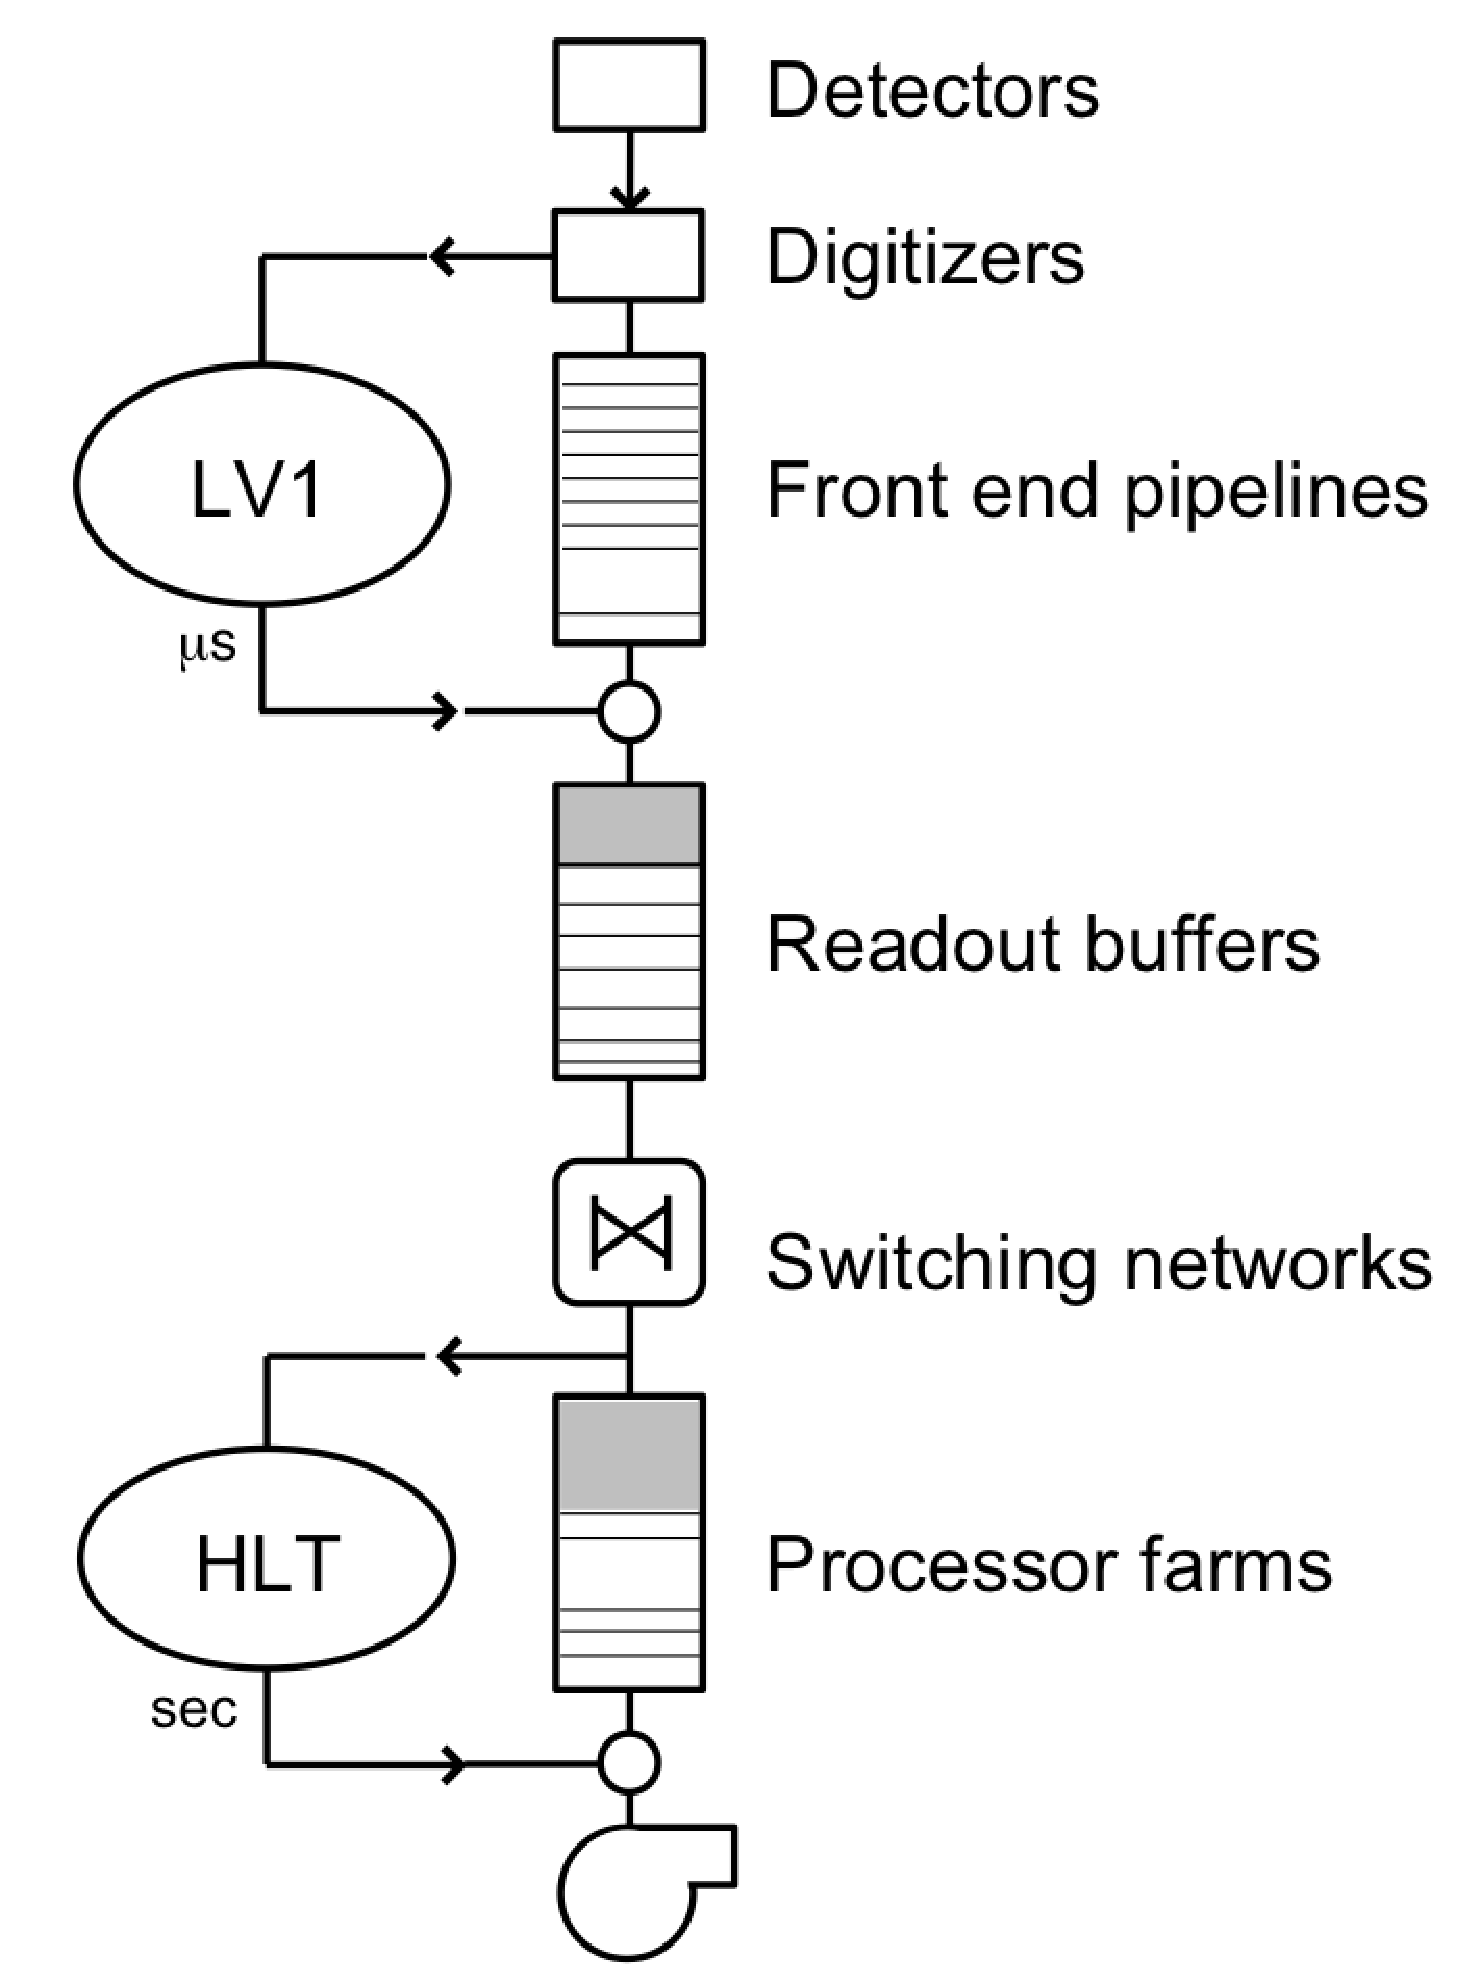
\includegraphics[width=0.4\textwidth]{daq_and_trig.pdf}
\caption{\label{fig:cms_daq}
Pictorial representation of the data acquisition system and
the flow of data from the CMS detector through both trigger levels~\cite{bourge}.
}
\end{center}
\end{figure}
% --------------------------------------------------------------------------- %

% --------------------------------------------------------------------------- %
% --------------------------------------------------------------------------- %
\section{Particle Reconstruction and Identification}
\label {sec:cms_reco}
% --------------------------------------------------------------------------- %
% --------------------------------------------------------------------------- %

The digitization of the events selected by the trigger only constitute
raw ingredients that need to be further processed in order to a give a
complete description of the particles present as the result of a proton-proton
collision. Many algorithms have been developed by the CMS collaboration to
reconstruct these particles; however, only the reconstruction algorithms used
in this thesis will be described here with a full description given in the
references. In this section we discuss charged particle, electron, muon, jet
and missing transverse energy reconstruction; which are the important objects
used in this analysis.

% --------------------------------------------------------------------------- %
% --------------------------------------------------------------------------- %
\subsection{Charged Particle Reconstruction}
\label {sec:cms_tracking}
% --------------------------------------------------------------------------- %
% --------------------------------------------------------------------------- %
Charged particles traversing the CMS detector first deposit energy in the
CMS tracker, leaving thousands of positional measurements to interpret
per bunch crossing. Determining the trajectory of these charged particles
amongst this collection of ``hits'' is an exercise in patter recognition.
Each charged particle can be described using five parameters that model
its trajectory as it is bent through the magnetic field. ``Tracking''
is the process of finding these ``tracks'' through the CMS tracking
system~\cite{pixel,mangano,trackingperformance}.

Individual silicon strip and pixel channels with a threshold above the
signal-to-noise ratio are clustered together based on proximity producing a
collection of positional measurements (along with the associated uncertainty).
These ``hits'' in the inner portion of the detector are used to seed multiple
tracking steps, each designed to find tracks from charged particles with
different properties. Each step takes an initial trajectory measurement
from the seed and propagates the trajectory from the inside to the outside
of the tracker using a combinatorial Kalman filter (CKF)~\cite{ckf}. After
propagation ends, the tracks are measured for quality and hits on high quality
tracks are removed from consideration before creating the seeds for the next
tracking step. The tracks produced with each step are then merged into a single
collection, eliminating duplicate tracks by comparing shared hits and keeping
tracks with higher quality.

The seeding step searches for combinations of two or three hits near the
beam line compatible with a particle trajectory with an energy above a given
threshold coming from the interaction point. The initial particle trajectory
is estimated using either a seed triplet or a seed pair and the beam spot.
There are seven tracking steps. The thresholds in each step is lowered
so that the initial steps have less background of seed candidates that lead
to tracks reconstructed for non-existent particles (fakes). The first two
steps are seeded using only triplets from the pixel detector, the second step
dropping the \pt threshold after the earlier higher \pt step. The third step
uses pairs of pixel hits to gain additional efficiency. The fourth step again
uses pixel triplets, but with a looser requirement on the compatibility with
the interaction point to search for displaced tracks and particles with longer
lifetimes. The fifth step again uses triplets, but allows for combinations
of hits in both the pixel and strip detectors. This allows for seeding of
particles which have slightly longer decay lengths or have a missed pixel hit
(due to detector inefficiency). The final two steps use pairs and triplets of
hits at further radii in the strip detector to search for particles which have
a large displacement.

In each step, after the seeds have been created, the initial trajectory
estimate is propagated inside-out, layer-by-layer through the detector using
the CKM algorithm. The algorithm accounts for losses of energy as the particle
traverse the material in the detector as well as the possibility of multiple
scatter. At each layer, the position of the trajectory is estimated and any
hits compatible with the position are added to the track. If more than one
compatible hit is found, multiple trajectories are kept and further propagated.
In addition, for each layer, a new trajectory is created assuming there is
no hit in the current layer to allow for detector inefficiency. The process
continues until either too many layers have been crossed without a hit or the
trajectory reaches the last layer of the tracker.

After the trajectories have been propagated, a final trajectory fit to the
collected hits is performed. Any outlying hits that fall too far from the
overall fit are removed. This gives a final accurate measurement of the tracks'
parameters. Vertex compatibility, number of hits in the track and the $\chi^2$
of the fit are used as quality control selections. Hits from tracks passing
tight quality selections are removed from consideration in subsequent tracking
steps.

After all seven steps have been performed, the resulting tracks from each step
are merged into a single collection. To ensure that no charged particles have
been reconstructed twice, any tracks that share a large fraction of its hists
are compared and only the best quality track is kept.

% --------------------------------------------------------------------------- %
% --------------------------------------------------------------------------- %
\subsection{Vertex Reconstruction}
\label {sec:cms_vertex}
% --------------------------------------------------------------------------- %
% --------------------------------------------------------------------------- %
In the high multiplicity environment of the LHC, it is essential to measure
the number of proton-proton interactions for each bunch crossing. Typically,
only one of the these interactions is responsible for the high \pt process
that triggered the event, and measuring the lepton impact parameters with
respect to the correct vertex is essential for the rejection of muons from
semi-leptonic flavor decays and electrons from photon conversions. Thus, a high
vertex reconstruction efficiency, a low fake vertex rate and the ability to
differentiate nearby interactions are all requirements needed for CMS's vertex
reconstruction.

Vertex reconstruction is performed in two steps. First, tracks are clustered
together using the deterministic annealing algorithm~\cite{davtx,dacms}. The
algorithm iteratively clusters tracks with nearby impact parameters first with
large windows and allowing a single track to be clustered multiple times.
Each iteration tightens the clustering window until a stopping condition is
met. Tracks are not allowed to cluster to vertices if their transverse impact
parameter is larger than 3 cm or the longitudinal impact parameter is larger
than 4 cm. The deterministic annealing algorithm was specifically choses due to
its high clustering efficiency even when faced with the noisy LHC environment.
Studies on the vertex efficiency show that the vertex reconstruction response
as a function of the number of interactions is linear.

The second step takes each cluster of tracks and fits the vertex position using
the adaptive vertex fitting algorithm \cite{vertexing,vtxfit}.  This algorithm
weighs tracks in the cluster based on compatibility with the vertex position
(and un-weights the tracks that are more incompatible) giving a good vertex
resolution of less than 50 \um depending on the number of tracks present in the
cluster.  More vertex reconstruction performance results can be found in
Reference~\cite{vtxtkres}.

% --------------------------------------------------------------------------- %
% --------------------------------------------------------------------------- %
\subsection{Electron Reconstruction}
\label {sec:cms_electron}
% --------------------------------------------------------------------------- %
% --------------------------------------------------------------------------- %

It is important to reconstruct and identify electrons efficiently and to
know their energy to a high precision. Electrons interact primarily via
the electromagnetic force and hence deposit a majority of their energy
in the ECAL. However, due to the large amount of material the electron
must traverse in the silicon tracker, the electron radiates a significant
amount of energy via bremsstrahlung and hence the ``footprint'' of the
electron's energy distribution is very complex. In addition, other particles
also leave a significant amount of energy in the ECAL, namely hadrons,
in particular the $\pi^0$, which decays predominantly to two photons .
Therefore, strong rejection of reconstructed electrons originating from
sources other than true electrons from the hard interaction (fakes) is needed
in the form of electron identification. The identification of electrons and
rejection of fake electrons are left to be presented in the context of this
analysis in Section~\ref{sec:evtsel_el} while the reconstruction algorithm is
summarized below. More information about electron reconstruction can be found
in References~\cite{baffiReco,egmReco,egm2013}.

The first step of electron reconstruction is to identify clusters of energy in
the ECAL, i.e. areas where many crystals in close proximity have large energy
deposits. As the electron travels through the silicon tracker, bremsstrahlung
causes losses of energy through radiated photons which then also deposit
energy in the ECAL. The strong magnetic field bends the electron in the
azimuthal direction and it will radiate energy, in the form of photons, which
will spread energy along $\phi$ in the ECAL. Therefore the footprint
of the electron is such that it is long in $\phi$ and narrow in $\eta$ and
multiple deposits of energy need to be clustered together to form a ``Super
Cluster (SC)'' containing the full amount of energy originally possessed by the
electron.

After all SCs have been assembled, electron reconstruction continues by
searching for the footprint of the electron in the tracker. Hits in the pixel
detector compatible with the energy-weighted center of the SC are
identified allowing for both positive and negative charge hypotheses. If two
or three compatible pixel hits are discovered, they are used to seed a track
building algorithm similar to that described in Section~\ref{sec:cms_tracking}.
The sole difference in the case of electrons is that track fitting is done with
a Gaussian sum filter (GSF)~\cite{gsf} algorithm which can handle the large
changes in electron trajectory due to bremsstrahlung.

In addition to this approach seeded by SCs, a separate algorithm is run in
parallel. This is a ``particle-flow'' based approach which will be described
in full in Section~\ref{sec:cms_pf}. Instead of first building a SC, the
algorithm searches for pixels seeds for all clustered energy. For each found
seed, the algorithm completes the trajectory building and then searches for
clusters to add to the electron. At each layer in the tracker along the
electron track, the position in the ECAL pointed to by the electron's current
momentum is used to search for additional compatible clusters that originate
from a radiated photon. After both algorithms are complete, the two collections
of electrons are merged. The SC seeded algorithm dominates at higher energies
($>20 \GeV$) while the track-seeded algorithm adds significant efficiency at
lower energies as well as in crowded environments such as near or inside a jet.
A graphic showing the different pieces of the two algorithms can be seen in
Figure~\ref{fig:cms_elereco}.

% --------------------------------------------------------------------------- %
\begin{figure}[tbhp]
\begin{center}
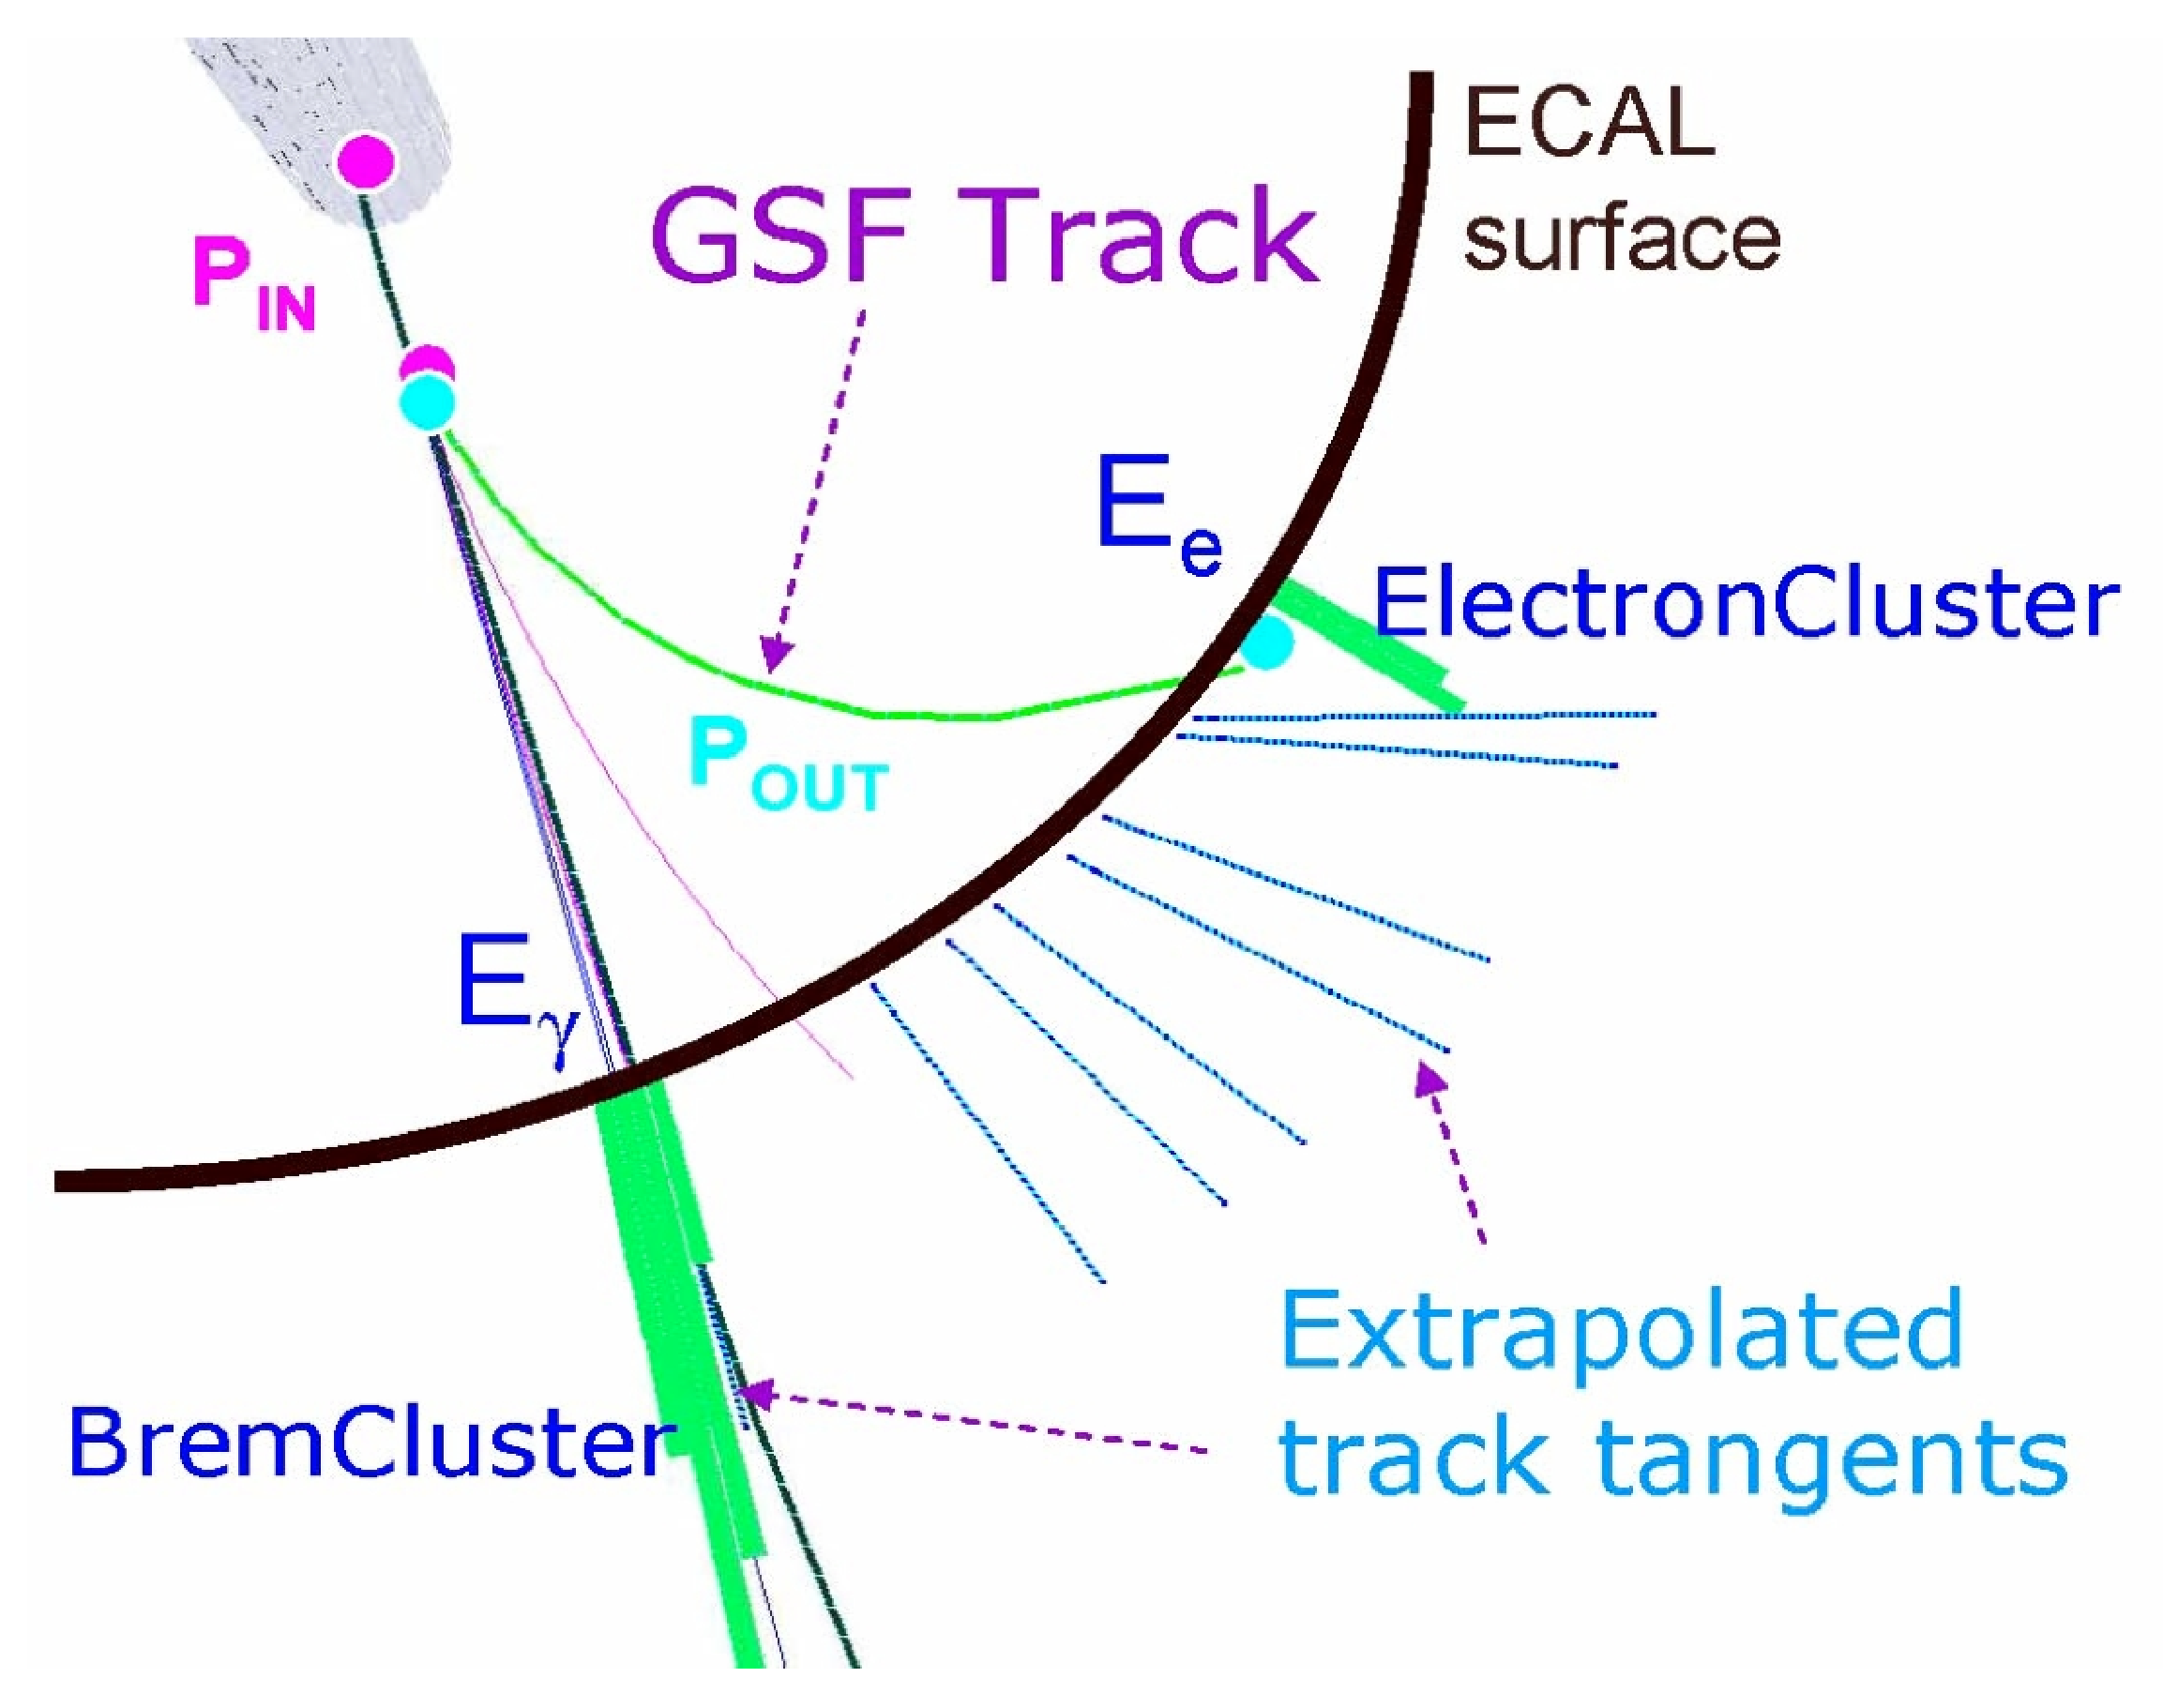
\includegraphics[width=0.6\textwidth]{elereco.pdf}
\caption[Depiction of the different portions of the electron reconstruction algorithm]
{\label{fig:cms_elereco}
Depiction of the different portions of the electron reconstruction algorithm.
Here the electron radiated a photon with a significant amount of energy early
in its traversal of the tracker and therefore there are two large clusters
(depicted in green) of energy present in the ECAL (depicted in black)~\cite{bourge}.
}
\end{center}
\end{figure}
% --------------------------------------------------------------------------- %

% --------------------------------------------------------------------------- %
% --------------------------------------------------------------------------- %
\subsection{Muon Reconstruction}
\label {sec:cms_muon}
% --------------------------------------------------------------------------- %
% --------------------------------------------------------------------------- %
Muons, in contrast to electrons, penetrate through to the outer regions of
the CMS detector due to their much higher mass and hence have a smaller
background contamination. Objects mis-reconstructed as muons in this
analysis come mostly from high energy hadrons which ``punch-through'' the
dense calorimeters and leave deposits in the muon detector. Another source
of background muons come from semi-leptonic decays of pions and kaons to
real muons. Reconstruction efficiency for muons is quite high and we can
therefore apply tight identification requirements to reduce these backgrounds
for this analysis. This is discussed in Section~\ref{sec:evtsel_mu}. The muon
reconstruction algorithm is discussed below, with more detailed information
available in References~\cite{muontdr,muonReco}.

Muon reconstruction begins by building segments in the muon sub-detector.
Positions of hits in the DT and CSCs are matched together to form small
segments compatible with a single particle passing through each chamber. Using
these segments (as well as hits in the RPCs) as positional measurements,
tracking is performed starting from the inside of the muon chamber and working
out to the outer edge of the muon system. Here, the Kalman Filter is used
to propagate and fit the muon tracks accounting for the loss of energy and
multiple scattering as the muon passes through the iron yoke. These tracks
built in the muon system are called ``Stand-Alone'' muons (SAM).

Since muons first passed through the CMS tracker, the SAMs are used to look
for tracks built in the silicon tracker matching the expected trajectory and
energy. Matched tracks are combined with the muon-only tracks and a global
refit is performed (again with the Kalman Filter algorithm). The resulting
muons are called ``global muons.''

In addition, another muon reconstruction algorithm is used to build muons
with information from the both the tracker and the muon system. ``Tracker''
muons are seeded from the tracks built in the silicon tracker. Each track is
extrapolated through both the ECAL and HCAL taking into account the expected
trajectory and uncertainty based on the magnetic field and the amount of
material it traverses. The energy deposited in the ECAL and HCAL at the expected
position of the muon's trajectory is checked to ensure compatibility with the
expectation from the minimum ionizing particle. The expected muon trajectory
is then extended into the muon system checking for matching segments. This
algorithm gives higher efficiency for lower \pt muons at the expense of a
larger background; however, muon identification selections can be applied for
further suppression.

% --------------------------------------------------------------------------- %
% --------------------------------------------------------------------------- %
\subsection{Particle Flow Reconstruction}
\label {sec:cms_pf}
% --------------------------------------------------------------------------- %
% --------------------------------------------------------------------------- %
The algorithms discussed up to this point have been the so-called
``detector-based'' algorithms. That is, reconstruction in each of the local
sub-detectors drives the higher level reconstruction of particles that leave their
signature in the respective sub-detectors. The ``particle-flow'' (PF) algorithm
is a paradigm shift from this type of algorithm in that it uses the very fine
segmentation of the CMS detector to search for an individual particle across
all the sub-detectors. For example, a charged hadron will leave a track in the
silicon tracker, a small amount of energy in the ECAL and will be deposited in
the HCAL, dissipating most of its energy. PF is used to identify particles in
this manner. When complete, the algorithm aims to have produced a list of all
the particles produced during the collision.

One large disadvantage of detector-based methods is the fact that energy
could be double counted, while with the PF algorithm, a global reconstruction
of the event is done on a particle-by-particle basis ensuring that double
counted energy is minimized. The resulting list of particles produced
by this algorithm is used extensively across many analyses at CMS. The
calculation of missing transverse energy (\met), jet reconstruction, and $\tau$
reconstruction are among the most important. The following briefly describes
the particle flow algorithm; however, a complete description can be found in
References~\cite{pfReco,pfComm}.

Before the PF reconstruction begins, local reconstruction in each of the
sub-detectors is completed and provides tracks from the silicon detector
(Section~\ref{sec:cms_tracking}), clustered energy in both the ECAL and HCAL
(similar to those discussed in Section~\ref{sec:cms_electron}) and the local
reconstruction product in the muon system (Section~\ref{sec:cms_muon}). The
general strategy is then to ``link'' these different inputs together to form
the complete picture of particles traversing through the detector. Objects
from each of the sub-detectors in close proximity are first grouped together
in blocks. Each block usually contains a few different inputs from each of the
detectors, i.e. a track pointing to an ECAL cluster, or an ECAL and HCAL energy
cluster adjacent to each other. Any blocks linked to signatures from isolated
muons or electrons are removed, as these have a very clean signature with very
little background. The blocks belonging to these particles (including the
clusters from radiated products as discussed in Section~\ref{sec:cms_electron})
are then removed from the list of unidentified blocks and added the list of PF
muons and electrons. Next, the momentum of any track pointing to calorimetric
clusters is compared to the energy contained in the ECAL or HCAL clusters.
If the energy and momentum of the two are compatible, the object is labeled
as a charged hadron, its energy is estimated as a weighted sum from both
objects, and its constituents are removed from the list and added to the list
of PF charged hadrons. If there is significantly more energy in the track
than is deposited in the calorimeter, a secondary muon identification is
performed searching for non-isolated lower \pt muons. If identified, again,
these constituents are removed and added to the PF muon list. If no muon is
found, tighter track requirements are applied to reject mis-reconstructed
tracks. If there is significantly more energy in the calorimeters, neutral
hadrons and photons are created comprising the energy unaccounted for by the
track. At this point, only unlinked clusters remain and all ECAL clusters are
hypothesized to be photons with all HCAL clusters hypothesized to be neutral
hadrons and added to their respective lists.

% --------------------------------------------------------------------------- %
% --------------------------------------------------------------------------- %
\subsection{Calculation of Missing Transverse Energy}
\label {sec:cms_met}
% --------------------------------------------------------------------------- %
% --------------------------------------------------------------------------- %
Neutrinos and other non-interacting particles from BSM theories, such
as neutralinos from supersymmetry, leave no signature as they traverse
the detector. Yet, we can infer their existence, transverse direction and
energy by looking at the sum of all of the transverse energy in the event.
As the two protons collide, all of their momentum is in the $z$-direction
(and negative-$z$), with no momentum transverse to the beam line. Momentum
conservation then requires that the transverse vectorial sum of all energy in
the event should sum to zero. If this calculation is performed and an imbalance
(missing transverse energy, \met) is detected, a non-interacting particle is
hypothesized to have escaped from the detector.

The \met reconstruction algorithm used by this analysis takes as input the full
collection of particle flow candidates and produces the negative vectorial sum.
Particle flow \met is defined as
\[
{\bf\met} =  - \displaystyle\sum_{i} {\bf \pt}^{i},
\]
where the summation is over all particles reconstructed with the particle
flow algorithm described in the previous section. Further information about
\met may be found in Reference \cite{metPerformance}.

% --------------------------------------------------------------------------- %
% --------------------------------------------------------------------------- %
\subsection{Jet Reconstruction}
\label {sec:cms_jets}
% --------------------------------------------------------------------------- %
% --------------------------------------------------------------------------- %
Jets are the experimental signatures of quarks and gluons produced in
high-energy processes such as proton-proton collisions. As quarks
and gluons have a net color charge and cannot exist freely due to
color-confinement, they are not directly observed in Nature. Instead, they
come together to form color-neutral hadrons, a process called hadronization
that leads to a collimated spray of hadrons called a jet.

Jet reconstruction is done by clustering nearby reconstructed PF
candidates. Starting with the highest \pt candidates as seeds, clustering is
done using the anti-$k_T$ algorithm~\cite{antikt} with a distance parameter of
$\DR=0.5$, defined in the $\eta-\phi$ plan. This clustering algorithm
uses a distance measurement inversely proportional to the square of each
particle's \pt and thus gives stability in the cases of infrared or collinear
radiation.

The use of PF candidates gives good jet energy response due to the high
reconstruction efficiencies of charged hadrons and photons which make up about
90\% of the jet's energy. However, some corrections are still applied to 
the jet energy with these energy scale corrections factorized into three steps.
First, an offset correction is applied to reduce the energy of the jet based on
the amount of pile-up in the event. A pile-up density is calculated using the
FastJet method~\cite{fastjet} to compute mean energy of jets in the event and
the ghost particle method for calculating jet areas~\cite{jetarea}.

Next, corrections for the detector response are made as a function of jet
\pt and $\eta$. The first portion of this correction is applied based on
measurements of simulated jet energies. The last correction is made to account
for the differences in the true CMS response between the physical and simulated
detector. The differences are measured by looking at jet energies in di-jet,
\gj and \Zj events where the object recoiling against the jet can be used to
measure the true jet energy. The uncertainty on this method is less that 5\%,
smaller than the overall jet energy resolution which ranges from 8\% to 15\%,
depending on the jet \pt and $\eta$. The remaining differences are explicitly
corrected for in data in the residual correction step, which completes the
jet energy correction chain. A full picture of jet reconstruction and energy
corrections can be found in Reference~\cite{cmsjetcal}.

% --------------------------------------------------------------------------- %
% --------------------------------------------------------------------------- %
\subsection{b-Jet Identification}                       \label {sec:cms_btags}
% --------------------------------------------------------------------------- %
% --------------------------------------------------------------------------- %

The identification of b-jets will be a major handle to select possible signal
event. One of the design requirements of the tracker was to find displaced
vertices of the long lived hadrons produced by b-quarks. Many algorithms were
designed to identify displaced vertices present in b flavored jets (b-jets);
however, we only discuss the one algorithm that is used in this analysis, the
Combined Secondary Vertex method (CSV)~\cite{btagging}.

The presence of a secondary vertex and the kinematic variables associated with
this vertex can be used to discriminate between a b and non-b jet. Two of these
variables are the distance and direction between the primary and secondary
vertices (the flight distance and direction). The significance of the flight
distance (the ratio of the flight distance to its estimated uncertainty) can be
used as a discriminating variable. In the CSV algorithm, the flight distance
information is combined with track-based lifetime information. By using this
additional information, the algorithm provides discrimination also in cases
where no secondary vertices are found, increasing the efficiency with respect
to using the secondary vertex information alone. The vertex category is defined
as
\begin{itemize}
  \item real: There exists a secondary vertex.
  \item pseudo: When no real vertex is found, tracks with a high impact parameter
significance ($S_{IP}$, the impact parameter divided by its uncertainty) are used
to create a ``pseudo'' vertex.
  \item no vertex: When no real or pseudo vertex is found.
\end{itemize}
In addition to the vertex category, the following variables are used to form a
discriminating variable (in the ``no vertex'' category, only the last two are
used):
\begin{itemize}
  \item the flight distance significance in the transverse plane (``2D'');
  \item the vertex mass;
  \item the number of tracks at the vertex;
  \item the ratio of the energy carried by the tracks at the vertex with respect to all tracks in the jet;
  \item the \pr of the tracks at the vertex with respect to the jet axis;
  \item the 2D $S_{IP}$ of the first track that raises the invariant mass above the charm threshold of 1.5\GeVcc;
  \item the number of tracks in the jet;
  \item the 3D $S_{IP}$ for each track in the jet.
\end{itemize}
A likelihood ratio is built from these variables. It is used to discriminate
between b and c jets and between b and light-parton jets. The distribution
of the CSV discriminator is shown in Figure~\ref{fig:cms_btag_disc}. In
this analysis, we use the ``medium'' working point, which is any jet with a
discriminator value greater than 0.679 is ``tagged'' as a b-jet.
% --------------------------------------------------------------------------- %
\begin{figure}[!hbt]
\begin{center}
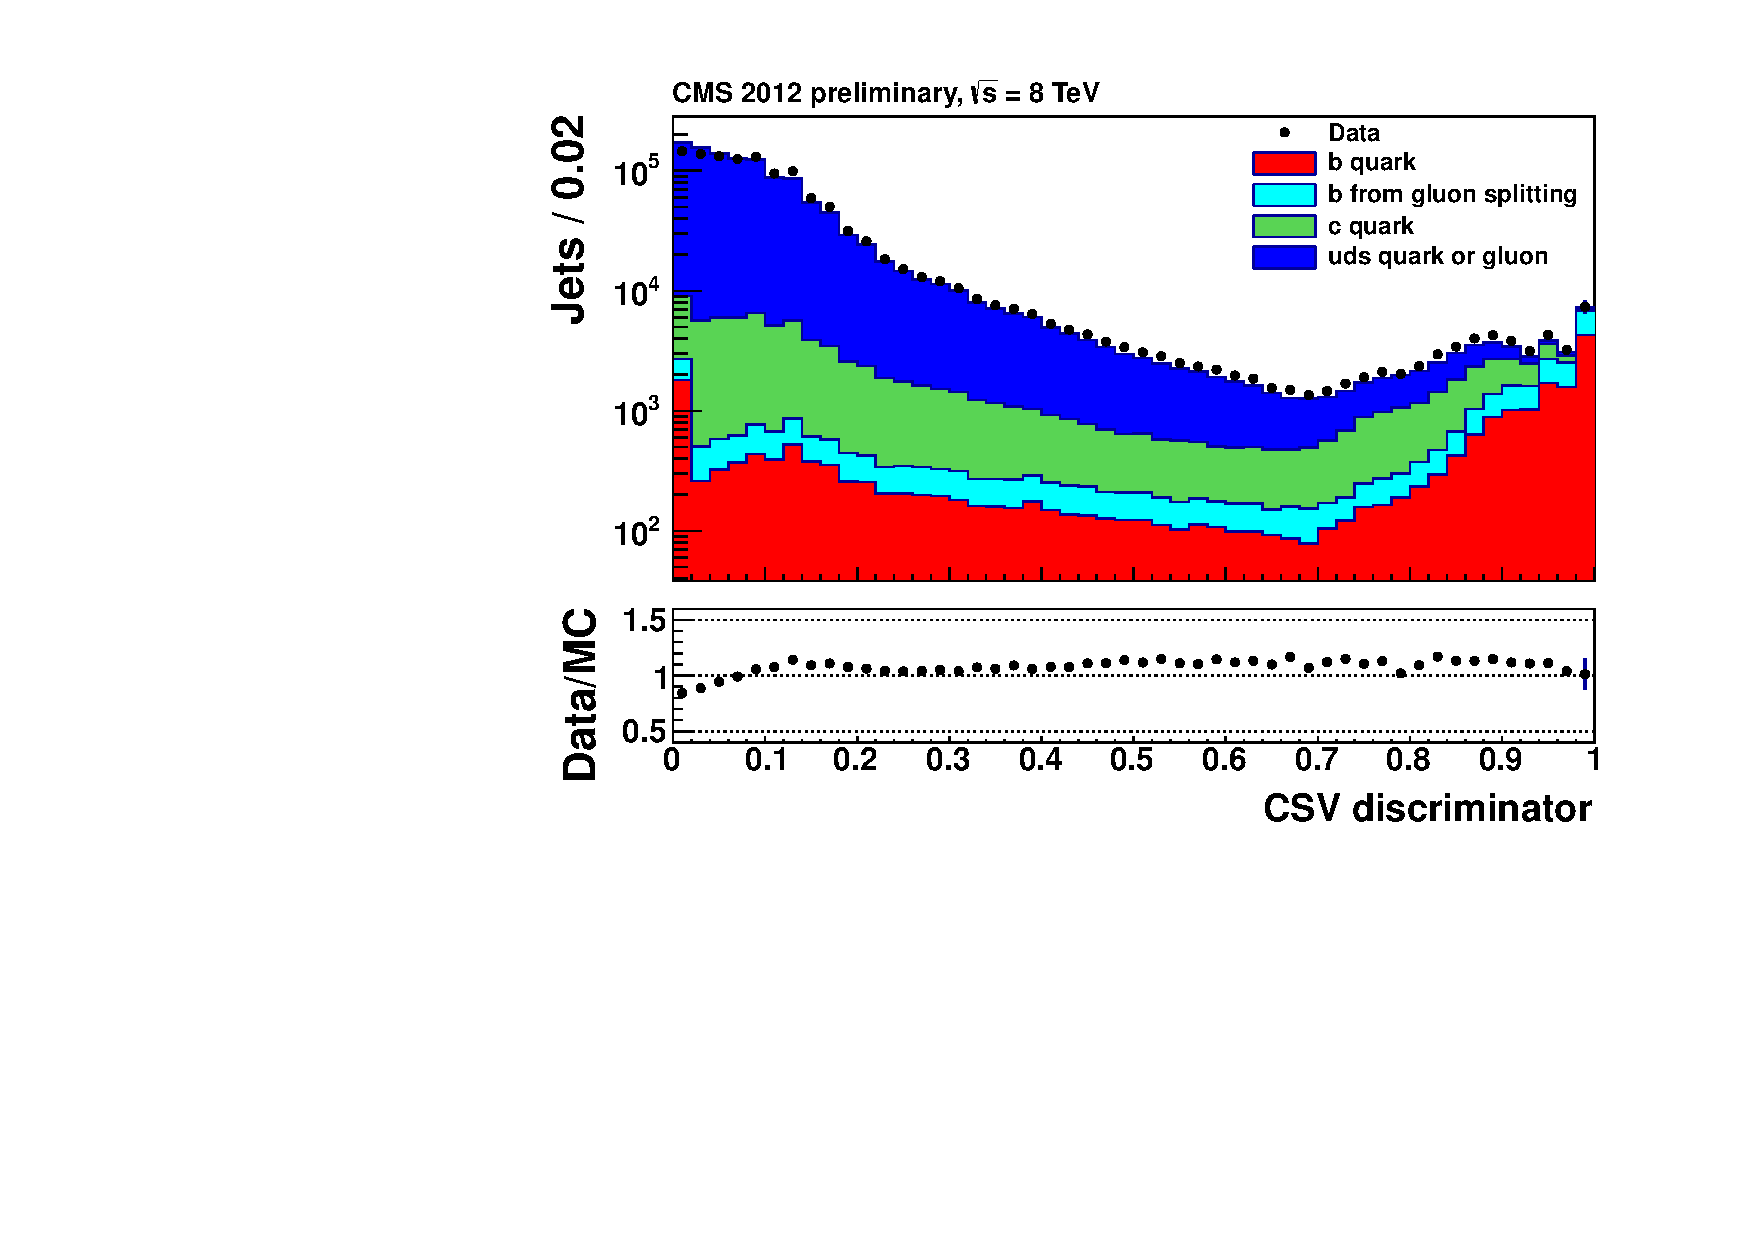
\includegraphics[width=0.7\textwidth]{btag_disc.pdf}
\caption[Combined Secondary Vertex algorithm discriminant for data and simulation.]
{\label{fig:cms_btag_disc}
Combined Secondary Vertex algorithm  discriminant for
data (black points) and compared to simulation of lighter flavor jets (green
and blue) as well as b-jets (cyan and red).  Larger values of the discriminant
are more indicative of heavy flavor jets.  The ratio between data and simulation
is shown at bottom~\cite{btagging}.
}
\end{center}
\end{figure} 
% --------------------------------------------------------------------------- %

% --------------------------------------------------------------------------- %
% \begin{figure}[!hbt]
% \begin{center}
% 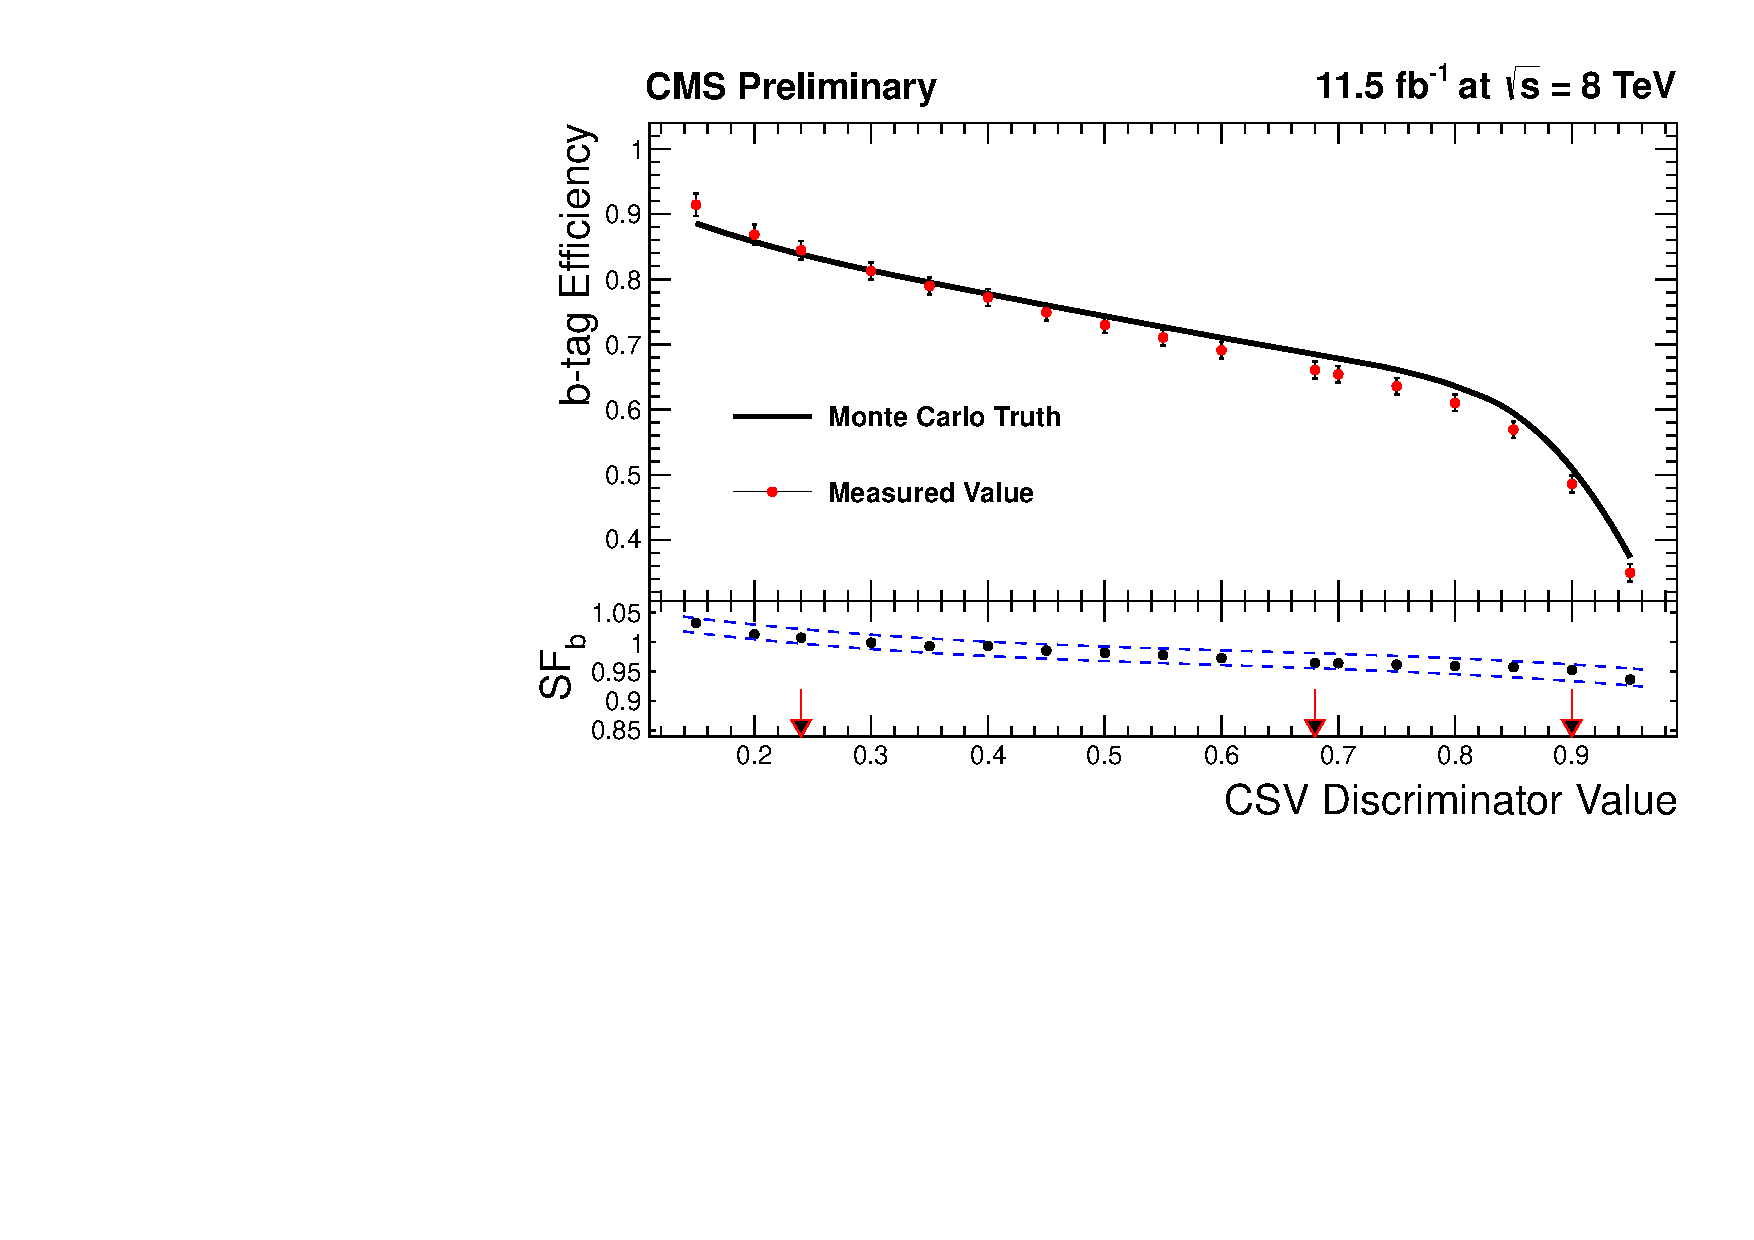
\includegraphics[width=0.7\textwidth]{btag_eff.pdf}
% \caption[b-jet efficiency for the track counting high effeciency b-tagging algorithm.]
% {\label{fig:cms_btag_eff}
% b-jet efficiency for the CSV algorithm in data (red points) and simulation
% (black line) as a function of the track counting high efficiency algorithm
% output discriminant. The ratio of data to simulation is plotted below with the
% blue band indicating the uncertainty on the measurement~\cite{btagging}.
% }
% \end{center}
% \end{figure} 
% --------------------------------------------------------------------------- %

